\documentclass[12pt, a4paper]{article}

\usepackage{FMF}

\newcommand{\naslov}{Logika in množice}

\renewcommand{\implies}{\Rightarrow}
\renewcommand{\iff}{\Leftrightarrow}

\makeindex

\begin{document}

\renewcommand{\headheight}{20pt}

\maketitle
\newpage
\tableofcontents

\newpage

\section*{Uvod}
\addcontentsline{toc}{section}{Uvod}
\markboth{Uvod}{}

V tem dokumenti so zbrani moji zapiski s predavanj predmeta Logika in množice v letu 2020/21. Predavatelj v tem letu je bil prof.~dr.~Marko Petkovšek.

Zapiski niso popolni. Manjka nekaj zgledov, ki pomagajo pri razumevanju definicij in izrekov. Poleg tega nisem dokazoval čisto vsakega izreka, pogosto sem ga označil kot očitnega ali pa le nakazal pomembnejše korake v dokazu.

Zelo verjetno se mi je pri pregledu zapiskov izmuznila kakšna napaka -- popravki so vselej dobrodošli.

\newpage

\section{Izjavni račun}

\epigraph{">Ta poved ni resnična."<}{---Paradoks o lažnivcu}

\subsection{Izjave in izjavni vezniki}

\begin{okvir}
\begin{definicija}
\emph{Izjava}\index{Izjava} je poved, ki je resnična ali neresnična.
\end{definicija}
\end{okvir}

\begin{zgled}
Resničnost izjav:

\begin{itemize}
\item Ena in ena je tri. - neresnična izjava
\item Ena in ena je dva. - resnična izjava
\item Koliko je ena in ena? - ni izjava
\item Ta poved ni resnična. - ni izjava
\end{itemize}
\end{zgled}

Izjave po vsebini delimo na resnične (resničnostna vrednost 1) in lažne (vrednost 0). Po obliki jih delimo na osnovne (ne vsebujejo izjavnih veznikov) in sestavljene.

\begin{zgled}
Osnovne in sestavljene izjave:

\begin{itemize}
\item Vreme je lepo. - osnovna
\item Vreme je lepo in Peter gre v hribe. - sestavljena
\item Če je vreme lepo, gre Peter v hribe. - sestavljena
\item Peter ne gre v hribe. - sestavljena
\end{itemize}
\end{zgled}

Resničnost sestavljene izjave je določena z resničnostjo njenih sestavnih delov.

\begin{definicija}
Naj bo $n\in\N=\set{0,~1,~2,~\dots}$. $n$-mestni \emph{izjavni veznik}\index{Izjavni veznik} je funkcija, ki vsaki urejeni $n$-terici ničel in enic priredi vrednost 0 ali 1. 
\end{definicija}

\begin{zgled}
Izjavni vezniki:

\setlength{\columnsep}{-2cm}
\begin{multicols}{2}
\begin{itemize}
\item Negacija, simbol: $\neg$
\item Konjunkcija, simbol: $\land$
\item Disjunkcija, simbol: $\lor$
\item Implikacija,\footnote{Če $p\implies q$, pravimo, da je $p$ \emph{antecedens}, $q$ pa \emph{konsekvens}.} simbol: $\implies$
\item Ekvivalenca, simbol: $\iff$
\item 0-mestna veznika 0 in 1
\end{itemize}

\columnbreak
\begin{table}[H]
\centering
\begin{tabular}{c|c|c|c|c|c|c}
$p$ & $q$ & $\neg p$ & $p\land q$ & $p\lor q$ & $p\implies q$ & $p\iff q$ \\
\hline 
0 & 0 & \multirow{2}{*}{1} & 0 & 0 & 1 & 1 \\
\cline{1-2}\cline{4-7} 
0 & 1 &  & 0 & 1 & 1 & 0 \\
\hline 
1 & 0 & \multirow{2}{*}{0} & 0 & 1 & 0 & 0 \\
\cline{1-2}\cline{4-7} 
1 & 1 &  & 1 & 1 & 1 & 1
\end{tabular}
\caption{\emph{Resničnostna tabela}\index{Resničnostna tabela} izjavnih veznikov}
\end{table}
\end{multicols}
\setlength{\columnsep}{10pt}
\end{zgled}

Vseh $n$-mestnih veznikov je $2^{2^n}$.

\newpage

\subsection{Izjavni izrazi}

\begin{okvir}
\begin{definicija}
Izjavni izrazi\index{Izjavni izraz}:

\begin{enumerate}[label=(\roman*)]
\item Vsaka izjavna konstanta je izjavni izraz
\item Vsaka izjavna spremenljivka $p_1,~p_2,~p_3,~\dots$ je izjavni izraz
\item Če je $f$ enomesten izjavni veznik in je $A$ izjavni izraz, je tudi $(fA)$ izjavni izraz
\item Če je $f$ dvomesten izjavni veznik in sta $A$ in $B$ izjavna izraza, je tudi $(AfB)$ izjavni izraz
\item Če je $f$ $n$-mesten izjavni veznik in so $A_1,~A_2,~\dots,~A_n$ izjavni izrazi, je tudi $f(A_1, A_2, \dots, A_n)$ izjavni izraz
\end{enumerate}
\end{definicija}
\end{okvir}

\begin{zgled}
Konstrukcijsko zaporedje za $((p\implies q)\land(\neg r))$:

\begin{multicols}{3}
\begin{enumerate}
\item $p$
\item $q$
\item $(p\implies q)$
\item $r$
\item $(\neg r)$
\item $((p\implies q)\land(\neg r))$
\end{enumerate}
\end{multicols}
\end{zgled}

\begin{definicija}
Dogovor o vrstnem redu veznikov:

\begin{enumerate}
\item $\neg$ ima prednost pred drugimi vezniki
\item Vsak veznik iz zaporedja ($\land,\lor,\implies,\iff$) ima prednost pred vezniki, ki so v tem zaporedju desno od njega
\item Če isti veznik nastopa večkrat, ima levi nastop prednost pred desnim
\item Zunanji par oklepajev izpuščamo
\end{enumerate}
\end{definicija}

Vsak izjavni izraz določa neko resničnostno tabelo in s tem tudi nek izjavni veznik.

\begin{zgled}\label{zg:1}
$f(p, q, r)=(p\implies q)\land\neg r$:

\begin{table}[H]
\centering
\begin{tabular}{ccc||ccc}
$p$ & $q$ & $r$ & $p\implies q$ & $\neg r$ & $(p\implies q)\land\neg r$ \\
\hline\hline
0 & 0 & 0 & 1 & 1 & 1 \\
0 & 0 & 1 & 1 & 0 & 0 \\
0 & 1 & 0 & 1 & 1 & 1 \\
0 & 1 & 1 & 1 & 0 & 0 \\
1 & 0 & 0 & 0 & 1 & 0 \\
1 & 0 & 1 & 0 & 0 & 0 \\
1 & 1 & 0 & 1 & 1 & 1 \\
1 & 1 & 1 & 1 & 0 & 0 \\
\end{tabular} 
\caption{Zgled \ref{zg:1}}
\end{table}
\end{zgled}

\newpage

\subsection{Tavtologije in enakovredni izrazi}

\begin{okvir}
\begin{definicija}
Izjavni izraz je

\begin{enumerate}
\item \emph{tavtologija}\index{Izjavni izraz!Tavtologija, protislovje}, če je resničen pri vseh naborih vrednosti svojih spremenljivk
\item \emph{protislovje}, če je neresničen pri vseh naborih vrednosti svojih spremenljivk
\item \emph{kontingenten}\index{Izjavni izraz!Kontingenten}, če ni tavtologija ali protislovje
\end{enumerate}
\end{definicija}
\end{okvir}

\begin{zgled}
Tavtologije in protislovja:

\begin{multicols}{2}
\begin{table}[H]
\begin{tabular}{cc||ccc}
$p$ & $q$ & $p\implies q$ & $\neg p\lor q$ & $p\implies q\iff\neg p\lor q$ \\
\hline\hline
1 & 1 & 1 & 1 & 1 \\
1 & 0 & 0 & 0 & 1 \\
0 & 1 & 1 & 1 & 1 \\
0 & 0 & 1 & 1 & 1 \\
\end{tabular}
\caption{Primer tavtologije}
\end{table}

\begin{table}[H]
\begin{tabular}{cc||ccc}
$p$ & $q$ & $q\implies p$ & $\neg(q\implies p)$ & $p\land\neg(q\implies p)$ \\
\hline \hline
1 & 1 & 1 & 0 & 0 \\
1 & 0 & 1 & 0 & 0 \\
0 & 1 & 0 & 1 & 0 \\
0 & 0 & 1 & 0 & 0 \\
\end{tabular}
\caption{Primer protislovja}
\end{table}
\end{multicols}

\begin{itemize}
\item 1, $p\lor\neg p$ in $p\implies(q\implies p)$ so primeri tavtologij
\item 0, $p\land\neg p$ in $p\land\neg(q\implies p)$ so primeri protislovij
\end{itemize}
\end{zgled}

\begin{definicija}
Izjavna izraza $A$ in $B$ sta \emph{enakovredna}\index{Izjavni izraz!Enakovredni izrazi}, če je $A\iff B$ tavtologija. S simboli to zapišemo $A\sim B$.
\end{definicija}

\begin{zgled}
Za poljubno izbiro $A$, $B$ in $C$ so naslednji izrazi enakovredni:

\begin{description}[align=left, labelwidth=\widthof{$A\lor(B\land C)\sim (A\lor B)\land(A\lor C)AA$}]
\item[$A\land 1\sim A$] idempotenca konjunkcije
\item[$A\lor A\sim A$] idempotenca disjunkcije
\item[$A\land B\sim B\land A$] komutativnost konjunkcije
\item[$A\lor B\sim B\lor A$] komutativnost disjunkcije
\item[$A\iff B\sim B\iff A$] komutativnost ekvivalence
\item[$A\land(B\land C)\sim(A\land B)\land C$] asociativnost konjunkcije
\item[$A\lor(B\lor C)\sim(A\lor B)\lor C$] asociativnost disjunkcije
\item[$A\iff(B\iff C)\sim(A\iff B)\iff C$] asociativnost ekvivalence
\item[$A\land(A\lor B)\sim A$] absorpcija konjunkcije glede na disjunkcijo
\item[$A\lor(A\land B)\sim A$] absorpcija disjunkcije glede na konjunkcijo
\item[$A\land(B\lor C)\sim (A\land B)\lor(A\land C)$] distributivnost konjunkcije glede na disjunkcijo
\item[$A\lor(B\land C)\sim (A\lor B)\land(A\lor C)$] distributivnost disjunkcije glede na konjunkcijo
\item[$\neg\neg A\sim A$] zakon dvojne negacije
\item[$\neg(A\land B)\sim \neg A\lor\neg B$] prvi De Morganov zakon
\item[$\neg(A\lor B)\sim \neg A\land\neg B$] drugi De Morganov zakon
\item[$A\implies B\sim\neg B\implies\neg A$] zakon kontrapozicije
\end{description}
\begin{align*}
A\land 0   &\sim 0     & 1\implies A&\sim A     & A\implies B      &\sim\neg A\lor B                      \\
A\land 1   &\sim A     & A\iff 0    &\sim\neg A & \neg(A\implies B)&\sim A\land\neg B                     \\
A\lor 0    &\sim A     & A\iff 1    &\sim A     & A\iff B          &\sim (A\implies B)\land(B\implies A)  \\
A\lor 1    &\sim 1     & A\implies A&\sim 1     & A\iff B          &\sim (\neg A\lor B)\land(A\lor\neg B) \\
A\implies 0&\sim\neg A & A\iff A    &\sim 1     & A\iff B          &\sim (A\land B)\lor(\neg A\land\neg B)\\
A\implies 1&\sim 1     & \neg 0     &\sim 1     & \neg(A\iff B)    &\sim\neg A\iff B                      \\
0\implies A&\sim 1     & \neg 1     &\sim 0     & \neg(A\iff B)    &\sim A\iff\neg B             
\end{align*}
\end{zgled}

\newpage

\subsection{Disjunktivna in konjunktivna normalna oblika}

\begin{okvir}
\begin{definicija}
Naj bo  $A$ kontingenten izjavni izraz in naj bo $T$ njegova resničnostna tabela.

\begin{enumerate}[label=(\roman*)]
\item \emph{Disjunktivna normalna oblika}\index{Disjunktivna normalna oblika} izraza $A$ je disjunkcija osnovnih konjunkcij,\footnote{\emph{Osnovna konjunkcija}\index{Osnovna konjunkcija in disjunkcija} $i$-te vrstice je konjunkcija tistih izjavnih spremenljivk, ki so tu resnične, in negacij tistih, ki so lažne.}
ki ustrezajo vrsticam tabele $T$, v katerih ima $A$ vrednost $1$.

\item \emph{Konjuktivna normalna oblika}\index{Konjunktivna normalna oblika} izraza $A$ je konjunkcija osnovnih disjunkcij,\footnote{\emph{Osnovna disjunkcija} $i$-te vrstice je disjunkcija tistih izjavnih spremenljivk, ki so tu lažne, in negacij tistih, ki so resnične.}
ki ustrezajo vrsticam tabele $T$, v katerih ima $A$ vrednost $0$. 
\end{enumerate}
\end{definicija}
\end{okvir}

\begin{trditev}
Če je $A$ kontingenten izraz, je $A\sim \text{DNO}(A)\sim \text{KNO}(A)$.
\end{trditev}

\obvs

\begin{zgled}\label{zg:2}
Podana je naslednja tabela:
\end{zgled}

\begin{wraptable}[9]{l}{0.4\textwidth}
\vspace{-0.7cm}
\centering
\begin{tabular}{ccc||c}
$p$ & $q$ & $r$ & $D$ \\
\hline\hline
1 & 1 & 1 & 0 \\
1 & 1 & 0 & 1 \\
1 & 0 & 1 & 0 \\
1 & 0 & 0 & 0 \\
0 & 1 & 1 & 0 \\
0 & 1 & 0 & 1 \\
0 & 0 & 1 & 0 \\
0 & 0 & 0 & 1 \\
\end{tabular}
\caption{Zgled \ref{zg:2}}
\end{wraptable}

\vspace{1cm}
$D$ mora biti resničen natanko v 2., 6. in 8. vrstici. Dovolj je tako nastaviti
\[
D=(p\land q\land\neg r)\lor(\neg p\land q\land\neg r)\lor(\neg p\land\neg q\land\neg r).
\]
Izraz lahko poenostavimo:
\begin{align*}
D&\sim ((p\land q)\lor(\neg p\land q)\lor (\neg p\land \neg q))\land\neg r
\\
&\sim ((p\lor \neg p)\land q\lor \neg p\land \neg q)\land\neg r
\\
&\sim (q\lor p)\land (q\lor q)\land\neg r
\\
&\sim (q\lor\neg p)\land\neg r
\\
&\sim(q\implies p)\land\neg r
\\
&\sim\neg(p\implies q\implies r)
\end{align*}

\newpage

\subsection{Sklepanje v izjavnem računu}

\begin{okvir}
\begin{definicija}
\emph{Sklep}\index{Sklep} je končno zaporedje izjav $p_1,~p_2,~\dots,~p_k,~z$, kjer so $p_i$ \emph{predpostavke}\index{Predpostavka} sklepa, $z$ pa zaključek. Sklep je \emph{pravilen} ali \emph{veljaven}, če je zaključek resničen vedno, ko so resnične vse predpostavke. Pišemo
\[
p_1,~p_2,~\dots,~p_k \models z.
\]
\end{definicija}
\end{okvir}

\begin{zgled}
Primer sklepa:

\begin{center}
\begin{tabular}{lcl}
Če je ta žival ptič, potem ima krila. && $p\implies q$
\\
Ta žival nima kril. && $\neg q$
\\
\cline{1-1}\cline{3-3}
Torej ta žival ni ptič. && $\neg p$
\end{tabular}
\end{center}
\end{zgled}

\begin{trditev}
Za vse izjavne izraze $A$, $B$ in $C$ velja

\begin{description}[align=left, labelwidth=\widthof{$A\implies B,~B\implies C \models A\implies CAA$}]
\item[$A,~A\implies B \models B$] modulus ponens (MP)
\item[$A\implies B,~\neg B \models \neg A$] modulus tollens (MT)
\item[$A\lor B,~\neg B \models A$] disjunktivni silogizem (DS)
\item[$A\implies B,~B\implies C \models A\implies C$] hipotetični silogizem (HS)
\item[$A\land B \models A$] poenostavitev (Po)
\item[$A,~B \models A\land B$] združitev (Zd)
\item[$A \models A\lor B$] pridružitev (Pr)
\end{description}
\end{trditev}

\begin{proof}
Pravilnost sledi iz pravilnostnih tabel.
\end{proof}

\begin{izrek}[Izrek o naravni dedukciji]\index{Izrek!O naravni dedukciji}
Naj bodo $A_1,~A_2,~\dots,~A_k$ izjavni izrazi. Če obstaja zaporedje izjavnih izrazov $B_1,~B_2,~\dots,~B_n$, tako da za vsak $i\in\set{1,2,\dots,n}$ velja vsaj ena izmed naslednjih možnosti:

\begin{enumerate}[label=\alph*)]
\item $B_i$ je eden od $A_j$,
\item $B_i$ je tavtologija,
\item $B_i\sim B_j$ za nek $j<i$ ali
\item $B_i$ logično sledi iz predhodnih izrazov $B_j$ po enem izmed osnovnih pravil sklepanja,
\end{enumerate}

potem $A_1,~A_2,~\dots,~A_k\models B_n$.
\end{izrek}

\obvs

Sklep ni pravilen, če obstaja taka izbira izjavnih spremenljivk, da so vse predpostavke resnične, zaključek pa ne.

\begin{zgled}\label{zg:3}
Ali $p\implies q,~p\lor r,~q\implies s,~r\implies t,~\neg s\models t$?
\begin{table}[H]
\centering
\begin{tabular}{c|c|l}
$i$ & $B_i$ & Utemeljitev \\
\hline
1 & $p\implies q$  & Predpostavka \\
2 & $p\lor r$      & Predpostavka \\
3 & $q\implies s $ & Predpostavka \\
4 & $r\implies t$  & Predpostavka \\
5 & $\neg s$       & Predpostavka \\
6 & $p\implies s$  & HS iz 1, 3 \\
7 & $\neg p$       & MT iz 6, 5 \\
8 & $r\lor p$      & $\sim 2$ \\
9 & $r$            & DS iz 8, 7 \\
10 & $t$           & MP iz 9, 4 \\
\end{tabular} 
\caption{Zgled \ref{zg:3}}
\end{table}
\end{zgled}

\begin{zgled}
Nepravilni sklep:

\begin{center}
\begin{tabular}{l}
Ta žival ima krila ali pa ni ptič.\\
Če je ta žival ptič, potem leže jajca.\\
\hline
Torej ta žival ne leže jajc.
\end{tabular}
\end{center}

Sklep ni pravilen, žival lahko ni ptič, nima kril in leže jajca. Našli smo \emph{protiprimer}\index{Protiprimer} -- vse predpostavke so resnične, zaključek pa ne.
\end{zgled}

\begin{izrek}\label{iz:1}
Sklep je pravilen natanko tedaj, ko je implikacija konjunkcije predpostavk in zaključka sklepa tavtologija.
\end{izrek}

\obvs

\begin{izrek}
$A_1,\dots,A_k\models B\implies C$ natanko tedaj, ko $A_1,\dots,A_k,B\models C$. Takemu sklepu pravimo \emph{pogojni sklep} (PS).
\end{izrek}

\begin{proof}
Naj bo $A=A_1\land A_2\land\dots\land A_k$. Uporabimo izrek \ref{iz:1}. Velja namreč
\[
A\implies(B\implies C)\sim \neg A\lor(\neg B\lor C)\sim(\neg A\lor\neg B)\lor C\sim \neg(A\land B)\lor C\sim A\land B\implies C.\qedhere
\]
\end{proof}

\begin{izrek}
$A_1,\dots,A_k\models B$ natanko tedaj, ko $A_1,\dots,A_k,\neg B\models 0$. Takemu sklepu pravimo \emph{sklep s protislovjem} (RA -- \emph{reductio ad absurdum}).
\end{izrek}

\begin{proof}
Naj bo $A=A_1\land A_2\land\dots\land A_k$. Znova uporabimo izrek \ref{iz:1}. Velja
\[
A\implies B\sim \neg A\lor B\sim \neg(A\land\neg B)\sim A\land\neg B\implies 0.\qedhere
\]
\end{proof}

\newpage

\subsection{Polni nabori izjavnih veznikov}

\begin{okvir}
\begin{definicija}
Množica $M$ izjavnih veznikov je \emph{poln nabor}\index{Poln nabor}, če za vsak izjavni izraz $A$ obstaja nek enakovreden izjavni izraz $B$, ki vsebuje le veznike iz $M$.
\end{definicija}
\end{okvir}

\begin{izrek}
$\set{\neg,\land,\lor}$ je poln nabor.
\end{izrek}

\begin{proof}
Vzamemo eno izmed normalnih oblik, $p\land\neg p$ ali $p\lor\neg p$.
\end{proof}

Da dokažemo, da je $M$ poln nabor, naredimo naslednje:

\begin{enumerate}
\item Izberemo nek znan poln nabor $P$
\item Vsak veznik iz $P$ izrazimo z vezniki iz $M$
\end{enumerate}

\begin{definicija}
Definiramo še naslednje dvomestne veznike:

\begin{itemize}
\item $p+q\sim\neg(p\iff q)$ -- stroga disjunkcija
\item $p\uparrow q\sim\neg(p\land q)$ -- Shefferjev veznik
\item $p\downarrow q\sim\neg(p\lor q)$ -- Łukasiewiczev veznik
\end{itemize}
\end{definicija}

Za zgornje izjavne veznike veljajo naslednje enakovrednosti:
\begin{align*}
& A+0\sim A     && A\uparrow 0\sim 1     && A\downarrow 0\sim\neg A \\
& A+1\sim\neg A && A\uparrow 1\sim\neg A && A\downarrow 1\sim 0     \\
& A+A\sim 0     && A\uparrow A\sim\neg A && A\downarrow A\sim\neg A
\end{align*}
\begin{description}[align=left, labelwidth=\widthof{$A+(B+C)\sim(A+B)+CAA$}]
\item[$A+B\sim B+A$] komutativnost stroge disjunkcije
\item[$A\uparrow B\sim B\uparrow A$] komutativnost Shefferjevega veznika
\item[$A\downarrow B\sim B\downarrow A$] komutativnost Łukasiewiczevega veznika
\item[$A+(B+C)\sim(A+B)+C$] asociativnost stroge disjunkcije
\end{description}

\begin{trditev}
Množice $\set{\neg,\land}$, $\set{\neg,\lor}$, $\set{\neg,\implies}$, $\set{0,\implies}$, $\set{1,+,\land}$, $\set{0,\iff,\lor}$, $\set{\uparrow}$ in $\set{\downarrow}$ so polni nabori.
\end{trditev}

\obvs

Kako pokazati, da neka množica $M$ ni poln nabor? Poiščemo \emph{invarianto}:\footnote{Invarianta je značilnost, ki ostane nespremenjena pri določenih transformacijah.}

\begin{definicija}
Naj bo $f$ $n$-mestni izjavni veznik.

\begin{enumerate}
\item $f$ \emph{ohranja vrednost 1}, če je $f(1,1,\dots,1)=1$.
\item $f$ \emph{ohranja vrednost 0}, če je $f(0,0,\dots,0)=0$.
\end{enumerate}
\end{definicija}

\begin{zgled}
Množici $\set{1,\land,\lor,\implies,\iff}$ in $\set{0,\land,\lor,+}$ nista polna nabora, saj prva ohranja 1, druga pa 0.
\end{zgled}

\newpage

\section{Predikatni račun}

\epigraph{">Takoj, ko gremo v realni svet, se zadeve zakomplicirajo."<}{---prof.~dr.~Marko Petkovšek}

\subsection{Motivacija}

\begin{zgled}
Z izjavnim računom ne moremo opisati celotne logike:

\begin{tabular}{l}
Vsak zajec ljubi korenje.\\
Feliks je zajec.\\
\hline
Torej Feliks ljubi korenje.
\end{tabular}

V zgornjem primeru nimamo izjavnih veznikov, sklep pa zato ni pravilen, saj izjave v formalnem smislu niso povezane. Definiramo dodatne simbole:

\begin{description}[labelwidth=1.5cm]
\item[$Z(x)$] $x$ je zajec
\item[$K(x)$] $x$ ljubi korenje
\item[$a$] Feliks
\item[$\forall x$] za vsak $x$
\end{description}

Zgornji sklep lahko tako formaliziramo:

\begin{tabular}{l}
$\forall x\colon(Z(x)\implies K(x))$\\
$Z(a)$\\
\hline
$K(a)$
\end{tabular}

Tu označimo

\begin{description}[labelwidth=1cm]
\item[$x$] individualna spremenljivka
\item[$a$] individualna konstanta
\item[$Z,K$] enomestna predikata
\item[$\forall x$] univerzalni kvantifikator
\item[$\colon()$] ločila
\end{description}
\end{zgled}

\begin{zgled}
S predikati lahko izrazimo več izjav:

\begin{enumerate}
\item
\begin{multicols}{2}
\begin{enumerate}
\item Vsi gasilci so hrabri.
\item Nekateri gasilci so hrabri.
\item Nekateri gasilci niso hrabri.
\item Noben gasilec ni hraber.
\end{enumerate}
\end{multicols}

Naj $G(x)$ označuje ">$x$ je gasilec"< in $H(x)$ označuje ">$x$ je hraber"<. Potem lahko zgornje izjave prevedemo v sledeče:

\begin{multicols}{2}
\begin{enumerate}
\item $\forall x\colon(G(x)\implies H(x))$
\item $\exists x\colon(G(x)\land H(x))$
\item $\exists x\colon(G(x)\land\neg H(x))$
\item $\forall x\colon(G(x)\implies\neg H(x))$
\end{enumerate}
\end{multicols}

\item Praštevil je neskončno mnogo. Ekvivalentno obstajajo poljubno velika praštevila.

Naj $P(x)$ označuje ">$p$ je praštevilo"< in naj $V(x,y)$ označuje $x>y$. Določimo še \emph{domeno}, ki je v tem primeru $\N$. Zgornjo izjavo lahko tako prevedemo v
\[
\forall n~\exists p\colon(V(p,n) \land P(p)).
\]
\item Naravno število $n$ je praštevilo, če in samo če ima natanko dva naravna delitelja.

Naj $E(x)$ označuje ">$x=y$"< in $f(x,y)$ označuje $x\cdot y$. Zgornjo izjavo lahko tako prevedemo v

\[
\forall x\colon(P(x)\iff V(x,1)\land \forall u~\forall v\colon (E(x,f(u,v))\implies E(u,1)\lor E(v,1))),
\]
oziroma
\[
\forall x\colon((P(x)\iff x>1\land \forall u~\forall v\colon(x=u\cdot v\implies u=1\lor v=1)).
\]
\end{enumerate}
\end{zgled}

\newpage

\subsection{Sintaksa}

\begin{enumerate}[label=\Alph*)]
\item Simboli:

\begin{enumerate}
\item individualne konstante: $a,b,c,\dots$
\item individualne spremenljivke: $x,y,z,\dots$
\item predikati: $P,Q,R,\dots$
\item funkcijski simboli: $f,g,h,\dots$
\item izjavni vezniki
\item simbola kvantifikacije
\end{enumerate}

\item Termi\index{Term}:

\begin{enumerate}
\item Vsaka individualna konstanta je term
\item Vsaka individualna spremenljivka je term
\item Naj bo $f$ neki $n$-mesten funkcijski simbol in $t_1,t_2,\dots,t_n$ termi. Potem je $f(t_1,t_2,\dots,t_n)$ term
\end{enumerate}

Term je \emph{zaprt}, če ne vsebuje individualnih spremenljivk.

\item Izjavne formule\index{Izjavna formula}:

\begin{enumerate}
\item Naj bo $P$ neki $n$-mesten predikat in $t_1,t_2,\dots,t_n$ poljubni termi. Potem je $P(t_1,t_2,\dots,t_n)$ izjavna formula. Taki formuli pravimo \emph{atomarna}.
\item Če je $F$ neki $n$-mesten izjavni veznik in so $\varphi_1,\varphi_2,\dots,\varphi_n$ izjavne formule. je tudi $F(\varphi_1,\varphi_2,\dots,\varphi_n)$ izjavna formula.
\item Če je $\varphi$ izjavna formula in $x$ poljubna individualna spremenljivka, sta $(\forall x\colon\varphi)$ in $(\exists x\colon\varphi)$ izjavni formuli. Pri tem je $\forall x$ \emph{univerzalni kvantifikator}\index{Kvantifikator} in $\exists x$ \emph{eksistenčni kvantifikator}, $\varphi$ pa doseg kvantifikatorja.
\end{enumerate}
\end{enumerate}

\begin{definicija}
Dogovor o prednostnem redu in opuščanju ločil:

\begin{enumerate}
\item Za izjavne veznike in zunanje oklepaje veljajo prejšnji dogovori
\item Kvantifikatorji imajo prednost pred izjavnimi vezniki
\item Ločila med zaporednimi kvantifikatorji opuščamo
\end{enumerate}
\end{definicija}

\begin{definicija}
Nastop neke individualne spremenljivke v izjavni formuli je \emph{vezan}, če je del nekega kvantifikatorja ali pa leži v dosegu nekega kvantifikatorja, ki vsebuje to spremenljivko, sicer pa je \emph{prost}.
\end{definicija}

\begin{definicija}
Izjavna formula je \emph{zaprta}, če so vsi nastopi individualnih spremenljivk v njej vezani.
\end{definicija}

Izjavno formulo $\varphi$ lahko zapišemo v obliki $\varphi(x)$, kjer je $x$ individualna spremenljivka. Če je $t$ term, s $\varphi(t)$ označimo izjavno formulo, ki jo dobimo iz $\varphi$, če \emph{vse} proste nastope $x$ v $\varphi$ zamenjamo s termom $t$ -- naredimo \emph{substitucijo}.

Izjavno formulo $\varphi$ lahko zapišemo kot $\varphi(x_1,x_2,\dots,x_n)$, kjer so $x_1,\dots,x_n$ \emph{različne} individualne spremenljivke. Če so $t_1,t_2,\dots,t_n$ termi, je $\varphi(t_1,t_2,\dots,t_n)$ izjavna formula, ki jo dobimo, če v $\varphi$ zamenjamo vse proste nastope $x_i$ s termom $t_i$ za $i=1,2,\dots,n$.

\newpage

\subsection{Semantika}

\begin{okvir}
\begin{definicija}
Naj bo $\mathcal{F}$ množica izjavnih formul, ki nas zanimajo. \emph{Interpretacijo}\index{Interpretacija} $I$ formul iz $\mathcal{F}$ podamo tako, da

\begin{enumerate}
\item izberemo \emph{neprazen} razred objektov $D$ (\emph{domena}\index{Domena} ali \emph{področje pogovora}),
\item vsaki individualni konstanti $a$ iz $\mathcal{F}$ priredimo nek $\overline{a}\in D$,
\item vsakemu $n$-mestnemu predikatu $P$ iz $\mathcal{F}$ priredimo neko $n$-mestno relacijo $\overline{P}$ v $D$,
\item vsakemu $n$-mestnemu funkcijskemu simbolu $f$ iz $\mathcal{F}$ priredimo preslikavo, ki vsako urejeno $n$-terico elementov domene $D$ preslika v natanko določen element $D$.
\end{enumerate}

Izjavne veznike interpretiramo enako kot prej, kvantifikatorja pa kot ">za vsak $x$ iz $D$"< in ">obstaja $x$ iz $D$"<.
\end{definicija}
\end{okvir}

\begin{zgled}
Podano imamo
\[
\mathcal{F}=\set{P(a),P(x),\forall x\colon P(x),P(f(a,b))}.
\]
Primer interpretacije:

\begin{itemize}
\item $D=\N$
\item $\overline{a}=2$, $\overline{b}=3$
\item $\overline{P}(x)\dots~x$ je praštevilo
\item $\overline{f}(x,y)=2x+y$
\end{itemize}

Potem je
\[
\overline{f(a,b)}=\overline{f}(\overline{a},\overline{b})=7.
\]

\begin{table}[H]
\centering
\begin{tabular}{l|l|l}
Izjavna formula $\varphi$ & Poved $\overline{\varphi}$ & Komentar \\
\hline 
$P(a)$                 & 2 je praštevilo                     & Resnična izjava \\
$P(x)$                 & $x$ je praštevilo                   & Ni izjava \\
$\forall x\colon P(x)$ & Vsako naravno število je praštevilo & Neresnična izjava \\
$P(f(a,b))$            & 7 je praštevilo                     & Resnična izjava \\
\end{tabular}
\caption{Interpretacija izjavnih formul}
\end{table}

">$x$ je praštevilo"< ni izjava, saj ji ne moremo določiti pravilnosti, dokler $x$ ne zavzame številske vrednosti.

Opazimo sledeče:

\begin{enumerate}
\item zaprtim termom ustrezajo elementi $D$,
\item vsaki izjavni formuli $\varphi$ ustreza neka poved $\overline{\varphi}$,
\item vsaki zaprti izjavni formuli $\varphi$ ustreza izjava $\overline{\varphi}$ o elementih $D$.
\end{enumerate}
\end{zgled}

\begin{zgled}\label{zg:4}
Podana je izjavna formula $\varphi=\forall x~\exists y\colon R(x,y)$.
\end{zgled}

\begin{table}[H]
\centering
\begin{tabular}{>{\raggedright}p{4.5cm}|p{6cm}|l}
Interpretacija & Izjava $\overline{\varphi}$ & Komentar \\
\hline 
$D=\N$, $\overline{R}(x,y)\dots x<y$ & Za vsako naravno število obstaja večje naravno število & Resnična izjava \\
$D=\N$, $\overline{R}(x,y)\dots x>y$ & Za vsako naravno število obstaja manjše naravno število  & Neresnična izjava \\
$D=\Z$, $\overline{R}(x,y)\dots x>y$ & Za vsako celo število obstaja manjše celo število  & Resnična izjava \\
$D=\set{\text{vsi ljudje}}$, $\overline{R}(x,y)\dots x$ ima rad $y$ & Vsak ima nekoga rad & Izjava \\
\end{tabular}
\caption{Zgled \ref{zg:4}}
\end{table}

Pogosto uporabljamo izjavne formule, ki niso zaprte. ">Tihi privzetek"< je, da je to izjavna formula, ki velja za vse individualne spremenljivke.
\begin{definicija}
Naj bo $\varphi$ izjavna formula in $x_1,\dots,x_n$ vse individualne spremenljivke, ki nastopajo v $\varphi$. Potem je
\[
z(\varphi)=\forall x_1\dots\forall x_n\colon \varphi
\]
\emph{univerzalno zaprtje}\index{Univerzalno zaprtje} formule $\varphi$.
\end{definicija}

\begin{definicija}
Izjavna formula $\varphi$ je \emph{resnična} v interpretaciji $I$, če je resnična izjava $\overline{z(\varphi)}$. Pišemo $I\models\varphi$.
\end{definicija}

\newpage

\subsection{Logično veljavne formule in enakovrednosti}

\begin{okvir}
\begin{definicija}
Izjavna formula $\varphi$ je

\begin{enumerate}
\item \emph{logično veljavna}, če je resnična v vseh možnih interpretacijah
\item \emph{protislovna}, če je neresnična v vseh interpretacijah
\end{enumerate}
\end{definicija}
\end{okvir}

\begin{zgled}
Naj bosta $P,Q$ enomestna predikata in $\varphi=(\forall x\colon P(x)\lor\forall x\colon Q(x)\implies\forall x\colon(P(x)\lor Q(x)))$. $\varphi$ je logično veljavna:

Naj bo $I$ poljubna interpretacija $\varphi$. Uporabimo pogojni sklep. Predpostavimo
\[I\models\forall x\colon P(x)\lor\forall x\colon Q(x).\]
Vzemimo poljuben $x_0\in D$. Ločimo dva primera:

\begin{enumerate}[label=\alph*)]
\item $I\models\forall x\colon P(x)$. Potem $I\models P(x_0)$
\item $I\models\forall x\colon Q(x)$. Potem $I\models Q(x_0)$
\end{enumerate}

Ker je $x_0\in D$ poljuben, sledi
\[
I\models\forall x\colon (P(x)\lor Q(x)).
\]
Ker je $I$ poljubna interpretacija, je $\varphi$ logično veljavna.\qed
\end{zgled}

\begin{zgled}
Naj bo $\psi=\forall x\colon(P(x)\lor Q(x))\implies \forall x\colon P(x)\lor\forall x\colon Q(x)$. $\psi$ ni logično veljavna. Kot protiprimer lahko namreč izberemo $D=\N$, $P(x)\dots$ $x$ je sod in $Q(x)\dots$ $x$ je lih.
\end{zgled}

\begin{zgled}
Naj bo $\chi=\exists y~\forall x\colon (R(x,y)\iff\neg R(x,x))$. $\chi$ je protislovje:


Naj bo $I$ poljubna interpretacija. Recimo $I\models\chi$. Torej obstaja $y_0$, da je $\forall x\colon(R(x,y_0)\iff\neg R(x,x))$. Sledi, da je $R(y_0,y_0)\iff\neg R(y_0,y_0)$, kar pa je protislovje. Ker je $I$ poljubna, je $\chi$ protislovna.
\end{zgled}

\begin{definicija}
Izjavni formuli $\varphi$ in $\psi$ sta \emph{enakovredni}\index{Izjavna formula!Enakovredne formule}, če je formula $\varphi\iff\psi$ logično veljavna. Pišemo $\varphi\sim\psi$.
\end{definicija}

\begin{izrek}
Naj bosta $\varphi,\psi$ poljubni izjavni formuli in $x,y$ poljubni individualni spremenljivki. Potem:

\begin{enumerate}
\item $\neg\forall x\colon \varphi\sim\exists x\colon\neg\varphi$
\item $\neg\exists x\colon\varphi\sim\forall x\colon\neg\varphi$
\item $\forall x~\forall y\colon\varphi\sim\forall y~\forall x\colon\varphi$
\item $\exists x~\exists y\colon\varphi\sim\exists y~\exists x\colon\varphi$
\item $\forall x\colon(\varphi\land\psi)\sim\forall x\colon\varphi\land\forall x\colon\psi$
\item $\exists x\colon(\varphi\lor\psi)\sim\exists x\colon\varphi\lor\exists x\colon\psi$
\item $\forall x\colon(\varphi\lor\psi)\sim\forall x\colon\varphi\lor\psi$, če $x$ ne nastopa prosto v $\psi$
\item $\exists x\colon(\varphi\land\psi)\sim\exists x\colon\varphi\land\psi$, če $x$ ne nastopa prosto v $\psi$
\item $\forall x\colon\varphi\sim\varphi$, če $x$ ne nastopa prosto v  $\varphi$
\item $\exists x\colon\varphi\sim\varphi$, če $x$ ne nastopa prosto v  $\varphi$
\item $\forall x\colon\varphi(x)\sim\forall y\colon\varphi(y)$, če $y$ ne nastopa v $\varphi(x)$
\item $\exists x\colon\varphi(x)\sim\exists y\colon\varphi(y)$, če $y$ ne nastopa v $\varphi(x)$
\end{enumerate}
\end{izrek}

\begin{definicija}
Za vsako izjavno formulo $\varphi$ obstaja enakovredna formula $\psi$, pri kateri vsi kvantifikatorji stojijo na začetku. Taki formuli pravimo \emph{preneksna oblika}\index{Izjavna formula!Preneksna oblika}.
\end{definicija}

\begin{zgled}
Izjavne formule lahko na naslednji način pretvorimo v preneksno obliko:

\begin{enumerate}[label=\alph*)]
\item
$\begin{aligned}[t]
\neg\forall x~\exists y\colon R(x,y)
&\sim\exists x\colon(\neg\exists y\colon R(x,y))
\\
&\sim\exists x~\forall y\colon\neg R(x,y)
\end{aligned}$
\item
$\begin{aligned}[t]
\exists x\colon P(x)\land\exists x\colon Q(x)
&\sim\exists x\colon P(x)\land\exists y\colon Q(y)
\\
&\sim\exists x\colon(\exists y\colon Q(y)\land P(x))
\\
&\sim\exists x~\exists y\colon(P(x)\land Q(y))
\end{aligned}$
\end{enumerate}
\end{zgled}

\newpage

\subsection{Sklepanje in dokazovanje v predikatnem računu}

\begin{okvir}
\begin{definicija}
Končno zaporedje izjavnih formul $\varphi_1,~\dots,~\varphi_k,~\psi$ je \emph{pravilen} ali \emph{veljaven sklep}\index{Sklep}, če je izjavna formula
\[
\varphi_1\land\dots\land\varphi_k\implies\psi
\]
logično veljavna.
\end{definicija}
\end{okvir}

\begin{zgled}
Velja
\[
P(a),\forall x\colon(P(x)\implies Q(x))\models Q(a).
\]
\end{zgled}

\begin{proof}
Naj bo $I$ poljubna interpretacija. Dokažimo, da
\[
I\models P(a)\land\forall x\colon(P(x)\implies Q(x))\implies Q(a).
\]
Uporabimo pogojni sklep. Privzemimo, da
\[
I\models P(a)\land\forall x\colon(P(x)\implies Q(x)),
\]
torej velja
\[
I\models P(a)\quad\text{in}\quad I\models\forall x\colon(P(x)\implies Q(x)).
\]
To pomeni, da
\[
I\models P(a)\implies Q(a),
\]
zato $I\models Q(a)$ (modus ponens). S tem je dokaz končan.
\end{proof}

\newpage

\section{Množica}

\epigraph{">Brijem vse tiste može iz mesta in samo tiste može, ki se ne brijejo sami."<}{---Paradoks o brivcu}

\subsection{Podajanje množic}

V teoriji množic je edini osnovni pojem \emph{množica}\index{Množica}. Vse druge matematične objekte lahko definiramo z množicami. Tako lahko na primer naravna števila definiramo na sledeč način:
\begin{align*}
0&=\emptyset
\\
1&=\set{0}
\\
2&=\set{0,1}
\\
&\vdots
\\
n+1&=\set{0,1,2,\dots,n}
\\
&\vdots
\end{align*}

V teoriji množic je osnovna relacija \emph{pripadnost}\index{Pripadnost} ($\in$).

\begin{okvir}
\textbf{Aksiom ekstenzionalnosti (AE):}\index{Aksiom!Ekstenzionalnosti}
\[
\forall x\colon(x\in A\iff x\in B)\implies A=B
\]
Če imata množici iste elemente, sta enaki.
\end{okvir}

Majhne končne množice lahko tako podamo z naštevanjem vseh elementov, na primer $A=\set{1,4,9}$. Sicer množice podamo z neko izjavno formulo $\varphi(x)$, kjer prosto nastopa le spremenljivka $x$: $A=\set{x\mid\varphi(x)}$. To je okrajšava za formulo
\[
\forall x\colon(x\in A\iff\varphi(x)).
\]
Russellovo vprašanje\index{Russellova antinomija}: Ali za množico $E=\set{x\mid x\not\in x}$ velja $E\in E$?

Po definiciji $E$ velja $E\in E\iff\varphi(E)\iff E\not\in E$. Naj bo
\[
\psi\colon\exists y~\forall x\colon(R(x,y)\iff\neg R(x,x)).
\]
Vzamemo interpretacijo $I$, pri kateri je $D=\set{x\mid x=x}$ razred vseh množic in $xRy\dots x\in y$. Vemo, da je $\psi$ protislovna, zato je $\neg\psi$ logično veljavna in resnična tudi v $I$. To pomeni, da
\[
\neg\exists E~\forall x\colon(x\in E\iff x\not\in x),
\]
torej Russellova množica ne obstaja.

Kako ">popraviti"< način podajanja množic?

\begin{enumerate}[label=\Alph*)]
\item \emph{NMG} (von~Neumann--Bernays--Gödel)\index{von~Neumann--Bernays--Gödelova teorija}:

Osnovni pojem je \emph{razred}\index{Razred}. Nekateri razredi so množice, drugi pa \emph{pravi razredi}. Razred $A$ je \emph{množica}, če $\exists B\colon A\in B$. Označimo $M(x)\dots x\text{ je množica}$. Množico $A$ podamo kot
\[
A=\set{x\mid\varphi(x)\land M(x)}.
\]
Vzemimo $R=\set{x\mid x\not\in x\land M(x)}$. Potem lahko izpeljemo $R\not\in R\land\neg M(R)$. $R$ je pravi razred.

\item \emph{ZFC} (Zermelo--Fraenklova teorija z aksiomom izbire)\index{Zermelo--Fraenklova teorija}:

Edini osnovni pojem je \emph{množica}. Privzamemo \emph{eksistenčne aksiome}, ki nam zagotavljajo obstoj dovolj ">majhnih"< množic.

Standardna interpretacija formul teorije ZFC:

\begin{itemize}
\item $D=V=\set{x;~x=x}$ je razred vseh množic
\item $x\in y$ je relacija pripadnosti
\item $x=y$ je relacija enakosti
\end{itemize}
\end{enumerate}

\newpage

\subsection{Relacije med množicami}

\subsubsection{Relacija enakosti}

Enakost v matematiki pojmujemo kot istost.

\begin{okvir}
\textbf{Načelo zamenljivosti enakega z enakim (EE):} Če je $A=B$, potem vse tisto, kar velja za $A$, velja tudi za $B$ in obratno.
\end{okvir}

\begin{trditev}
$A=B\iff\forall x\colon(x\in A\iff x\in B)$.
\end{trditev}

\begin{proof}
Trditev je direktna posledica aksioma ekstenzionalnosti in načela zamenljivosti enakega z enakim.
\end{proof}

\begin{posledica}
Veljajo naslednje lastnosti:

\begin{enumerate}[label=(\roman*)]
\item $A=A$ (refleksivnost)
\item $A=B\implies B=A$ (simetričnost)
\item $A=B\land B=C\implies A=C$ (tranzitivnost)
\end{enumerate}
\end{posledica}

\obvs

\newpage

\subsubsection{Relacija inkluzije}

\begin{okvir}
\begin{definicija}
\emph{Relacija inkluzije}\index{Relacija inkluzije} ($\subseteq$) je definirana kot
\[
A\subseteq B\iff\forall x\colon(x\in A\implies x\in B).
\]
To preberemo kot ">$A$ je \emph{podmnožica}\index{Množica!Podmnožica} $B$"<. Namesto $\neg(A\subseteq B)$ pišemo $A\not\subseteq B$.
\end{definicija}
\end{okvir}

\begin{trditev}
$A=B\iff(A\subseteq B\land B\subseteq A)$.
\end{trditev}

\obvs

\begin{okvir}
\textbf{Aksiomska shema o podmnožicah (ASP)\index{Aksiom!Shema o podmnožicah}:} Če $B$ obstaja in je $\varphi(x)$ izjavna formula, v kateri prosto nastopa le $x$, obstaja tudi množica
\[
A=\set{x\mid x\in B\land \varphi(x)},
\]
oziroma
\[
\forall B~\exists A~\forall x\colon(x\in A\iff x\in B\land\varphi(x)).
\]
\end{okvir}

\begin{definicija}
Množica $A$ je \emph{prazna}\index{Množica!Prazna}, če $\forall x\colon x\not\in A$.
\end{definicija}

\begin{posledica}
Prazna množica obstaja. Imamo namreč množico $A$, za katero je
\[
\forall B~\exists A~\forall x\colon(x\in A\iff x\in B\land x\ne x),
\]
od koder sledi $\exists A~\forall x\colon x\not\in A$.
\end{posledica}

\begin{posledica}
Razred vseh množic $V$ ni množica (je pravi razred).
\end{posledica}

\begin{proof}
Predpostavimo, da je $V$ množica. Potem obstaja $A=\set{x\mid x\in V\land x\not\in x}$, kar je protislovje.
\end{proof}

\begin{okvir}
\textbf{Aksiom o paru (AP)\index{Aksiom!O paru}:} Če obstajata $u$ in $v$, obstaja tudi
\[
A=\set{u,v}=\set{x\mid x=u\lor x=v}.
\]
\end{okvir}

\begin{posledica}
Če obstaja $u$, obstaja $A=\set{u}$.
\end{posledica}

\begin{proof}
V aksiomu o paru vzamemo $u=v$.
\end{proof}

\begin{izrek}
Veljajo naslednje lastnosti:

\begin{enumerate}[label=(\roman*)]
\item $A\subseteq A$ (refleksivnost)
\item $A\subseteq B\land B\subseteq A\implies A=B$ (antisimetričnost)
\item $A\subseteq B\land B\subseteq C\implies A\subseteq C$ (tranzitivnost)
\item $\emptyset\subseteq A$
\item $A\subseteq\emptyset\implies A=\emptyset$
\end{enumerate}
\end{izrek}

\obvs

\newpage

\subsubsection{Relacija stroge inkluzije}

\begin{okvir}
\begin{definicija}
\emph{Relacija stroge inkluzije}\index{Relacija stroge inkluzije} ($\subset$) je definirana kot
\[
A\subset B\iff A\subseteq B\land A\ne B.
\]
Pravimo, da je $A$ \emph{prava podmnožica} $B$. Namesto $\neg(A\subset B)$ pišemo $A\not\subset B$.
\end{definicija}
\end{okvir}

\begin{trditev}
Velja $A\subset B\iff A\subseteq B\land \exists x\colon(x\in B\land x\not\in A)$.
\end{trditev}

\obvs

\begin{izrek}
Za vse množica $A$, $B$ in $C$ velja:

\begin{enumerate}[label=(\roman*)]
\item $A\not\subset A$ (irefleksivnost)
\item $A\subset B\implies B\not\subset A$ (asimetričnost)
\item $A\subset B\land B\subset C\implies A\subset C$ (tranzitivnost)
\end{enumerate}
\end{izrek}

\obvs

\newpage

\subsection{Operacije z množicami}

\subsubsection{Unija, presek, razlika, Boolova vsota}

\begin{okvir}
\begin{definicija}
Definiramo naslednje operacije:

\begin{description}[align=left, labelwidth=\widthof{$A\setminus B$}+\widthof{$A\oplus B=\set{x\mid x\in A+x\in B}A$}]
\item[\hspace{\widthof{$A\setminus B$}}$A\cup B=\set{x\mid x\in A\lor x\in B}$] --\emph{unija}\index{Unija}
\item[\hspace{\widthof{$A\setminus B$}}$A\cap B=\set{x\mid x\in A\land x\in B}$] --\emph{presek}\index{Presek}
\item[\hspace{\widthof{$A\cup B$}}$A\setminus B=\set{x\mid x\in A\land x\not\in B}$] --\emph{razlika}\index{Razlika}
\item[\hspace{\widthof{$A\setminus B$}+\widthof{$A\cup B$}-\widthof{$A\oplus B$}}$A\oplus B=\set{x\mid x\in A+x\in B}$] --\emph{Boolova vsota} ali --\emph{simetrična razlika}\index{Boolova vsota}
\end{description}
\end{definicija}
\end{okvir}

\begin{trditev}
Za poljubni množici $A$ in $B$ obstajata $A\cap B$ in $A\setminus B$.
\end{trditev}

\obvs

\begin{izrek}
Za vse množice $A$, $B$ in $C$ velja:

\begin{enumerate}[label=(\roman*)]
\item Operacije s prazno množico:

\vspace{-6pt}
\begin{multicols}{3}
\begin{itemize}
\item $A\cup\emptyset = A$
\item $A\cap\emptyset=\emptyset$
\item $A\setminus\emptyset=A$
\item $\emptyset\setminus A=\emptyset$
\item $A\oplus\emptyset=A$
\end{itemize}
\end{multicols}
\vspace{-12pt}

\item Idempotenci:

\vspace{-6pt}
\begin{multicols}{3}
\begin{itemize}
\item $A\cup A=A$ 
\item $A\cap A=A$
\end{itemize}
\end{multicols}
\vspace{-12pt}

\item Komutativnosti:

\vspace{-6pt}
\begin{multicols}{3}
\begin{itemize}
\item $A\cup B=B\cup A$
\item $A\cap B=B\cap A$
\item $A\oplus B=B\oplus A$
\end{itemize}
\end{multicols}
\vspace{-12pt}

\item Asociativnosti:

\begin{itemize}
\item $(A\cup B)\cup C=A\cup(B\cup C)$ 
\item $(A\cap B)\cap C=A\cap (B\cap C)$
\item $(A\oplus B)\oplus C=A\oplus(B\oplus C)$
\end{itemize}

\item Absorpciji:

\vspace{-6pt}
\begin{multicols}{3}
\begin{itemize}
\item $A\cup(A\cap B)=A$
\item $A\cap(A\cup B)=A$
\end{itemize}
\end{multicols}
\vspace{-12pt}

\item Distributivnosti:

\begin{itemize}
\item $A\cup(B\cap C)=(A\cup B)\cap(A\cup C)$
\item $A\cap(B\cup C)=(A\cap B)\cup(A\cap C)$
\item $A\cap(B\oplus C)=(A\cap B)\oplus(A\cap C)$
\end{itemize}

\item Monotonosti:

\vspace{-6pt}
\begin{multicols}{2}
\begin{itemize}
\item $A\subseteq B\implies A\cup C\subseteq B\cup C$
\item $A\subseteq B\implies A\cap C\subseteq B\cap C$
\end{itemize}
\end{multicols}
\vspace{-12pt}

\item $A\oplus B=(A\setminus B)\cup(B\setminus A)=(A\cup B)\setminus(A\cap B)$
\item $A\cap B\subseteq A\subseteq A\cup B$
\item $A\subseteq B\iff A\cup B=B\iff A\cap B=A\iff A\setminus B=\emptyset$
\end{enumerate}
\end{izrek}

\obvs

\begin{definicija}
Naj bo $A$ množica in $\varphi$ izjavna formula. Potem sta formuli
\[
\forall x\in A\colon\varphi\qquad\text{in}\qquad\exists x\in A\colon\varphi
\]
okrajšavi za $\forall x\colon(x\in A\implies\varphi)$ in $\exists x\colon(x\in A\land\varphi)$ zaporedoma.
\end{definicija}

\begin{opomba}
Če $A\ne\emptyset$, za kvantifikatorja $\forall x\in A$ in $\exists x\in A$ veljajo analogne enakovrednosti kot za $\forall x$ in $\exists x$.
\end{opomba}

\begin{definicija}
Naj bo $A$ neprazna množica. Potem je
\[
\bigcup A=\set{x\mid \exists y\in A\colon x\in y}\qquad\text{in}\qquad\bigcap A=\set{x\mid \forall y\in A\colon x\in y}
\]
\end{definicija}

\begin{trditev}
$\forall y\in A\colon y\subseteq\bigcup A$ in $\forall y\in A\colon\bigcap A\subseteq y$ za neprazen $A$.
\end{trditev}

\obvs

\begin{okvir}
\textbf{Aksiom o uniji (AU)\index{Aksiom!O uniji}:}
\[
\forall A~\exists B~\forall x\colon(x\in B\iff\exists y\in A\colon x\in y)
\]
Za vsako množico $A$ obstaja njena unija.
\end{okvir}

\begin{posledica}
Za poljubni množici $A$ in $B$ obstajata množici $A\cup B$ in $A\oplus B$.
\end{posledica}

\begin{proof}
Obstaja unija $\set{A,B}$, ki obstaja po aksiomu o paru. Ker velja $A\oplus B\subseteq A\cup B$, smo končali.
\end{proof}

\begin{trditev}
Naj bo $A\ne\emptyset$. Potem obstaja $\bigcap A$.
\end{trditev}

\begin{proof}
Vzemimo poljuben element $y_0\in A$. Potem obstaja množica
\[
P=\set{x\mid x\in y_0\land \forall y\in A\colon x\in y}=\set{x\mid\forall y\in A\colon x\in y}=\bigcap A.\qedhere
\]
\end{proof}

\newpage

\subsubsection{Komplement množice}

Pogosto se omejimo na neko \emph{univerzalno množico}\index{Univerzalna množica} ali \emph{svet} $S$ in gledamo le njene podmnožice.

\begin{okvir}
\begin{definicija}
Naj bo $A\subseteq S$. \emph{Komplement množice}\index{Množica!Komplement} $A$ je definiran kot
\[
A^\mathsf{c}=\set{x\in S\mid x\not\in A}=S\setminus A.
\]
\end{definicija}
\end{okvir}

\begin{izrek}
Za vse $A,B,C\subseteq S$ velja:

\begin{enumerate}
\item $(A^\mathsf{c})^\mathsf{c}=A$
\item $(A\cup B)^\mathsf{c}=A^\mathsf{c}\cap B^\mathsf{c}$
\item $(A\cap B)^\mathsf{c}=A^\mathsf{c}\cup B^\mathsf{c}$
\item $A\setminus B=A\cap B^\mathsf{c}$
\item $A\subseteq B\iff B^\mathsf{c}\subseteq A^\mathsf{c}$
\item $A\cap B=\emptyset\iff A\subseteq B^\mathsf{c}\iff B\subseteq A^\mathsf{c}$
\item $A\cup A^\mathsf{c}=S$, $A\cap A^\mathsf{c}=\emptyset$
\item $A\cup S=S$, $A\cap S=A$
\end{enumerate}
\end{izrek}

\obvs

\begin{opomba}
Za $A\subseteq S$ lahko definiramo
\[
\bigcap A=\set{x\in S\mid \forall y\in A\colon x\in y}.
\]
Potem je
\[
\bigcap\emptyset=\set{x\mid x\in S}=S.
\]
\end{opomba}

\newpage

\subsubsection{Potenčna množica}

\begin{okvir}
\begin{definicija}
\emph{Potenčna množica}\index{Množica!Potenčna} množice $A$ je definirana kot
\[
\pot A=\set{x\mid x\subseteq A}.
\]
\end{definicija}
\end{okvir}

\begin{opomba}
Velja ekvivalenca
\[
x\in\pot A\iff x\subseteq A.
\]
\end{opomba}

\begin{okvir}
\textbf{Aksiom o potenčni množici (APM):}\index{Aksiom!O potenčni množici}
\[
\forall A~\exists B~\forall x\colon(x\in B\iff x\subseteq A)
\]
Za vsako množico $A$ obstaja njena potenčna množica.
\end{okvir}

\begin{izrek}
Za vse $A,B$ velja

\begin{enumerate}
\item $\emptyset\in\pot A$, $A\in\pot A$
\item $\bigcup\pot A=A$, $\bigcap\pot A=\emptyset$
\item $A\subseteq B\implies \pot A\subseteq\pot B$
\item $\pot A\cap\pot B=\pot (A\cap B)$
\item $\pot A\cup\pot B\subseteq \pot (A\cup B)$
\end{enumerate}
\end{izrek}

\obvs

\newpage

\subsubsection{Urejeni pari in kartezični produkt}

\begin{okvir}
\begin{definicija}
\emph{Urejen par}\index{Urejen par} definiramo kot
\[
(a,b)=\set{\set{a,b},\set{a}}.
\]
\end{definicija}
\end{okvir}

\begin{izrek}
Za vse $a,b,c,d$ velja
\[
(a,b)=(c,d)\iff a=c\land b=d.
\]
\end{izrek}

\begin{proof}
Če je $a=c$ in $b=d$, je očitno $(a,b)=(c,d)$. Zdaj predpostavimo, da je $(a,b)=(c,d)$. To pomeni, da je
\[
\set{\set{a,b},\set{a}}=\set{\set{c,d},\set{c}}.
\]
Sledi, da je $\set{a}=\set{c}$ ali $\set{a}=\set{c,d}$. V obeh primerih sledi $a=c$. Zdaj ločimo dva primera:

\begin{enumerate}
\item $a=b$: Sledi, da je
\[
\set{\set{a,d},\set{a}}=\set{\set{a,b},\set{a}}=\set{\set{a}},
\]
torej je $d=a$ in $a=b=c=d$.
\item $a\ne b$: Ker je
\[
\set{\set{a,b},\set{a}}=\set{\set{a,d},\set{a}},
\]
je $\set{a,b}=\set{a}$ ali $\set{a,d}$. Ker $b\ne a$, je edina možnost $b=d$.\qedhere
\end{enumerate}
\end{proof}

\begin{trditev}
Za vse $a,b$ obstaja $(a,b)$.
\end{trditev}

\begin{proof}
Dvakrat uporabimo aksiom o paru.
\end{proof}

\begin{okvir}
\begin{definicija}
Množica vseh parov, kjer prva komponenta pripada $A$, druga pa $B$,je \emph{kartezični produkt}\index{Kartezični produkt} množic $A$ in $B$:
\[
A\times B=\set{(x,y)\mid x\in A\land y\in B}.
\]
\end{definicija}
\end{okvir}

\begin{trditev}
Za poljubni množici $A$ in $B$ obstaja $A\times B$.
\end{trditev}

\begin{proof}
Dovolj je opaziti $A\times B\subseteq\mathcal{PP}(A\cup B)$. Velja namreč
\begin{align*}
A\times B&=\set{x\mid x\in\mathcal{PP}(A\cup B)\land \exists u~\exists v\colon(u\in A\land v\in B\land x=(u,v))}
\\
&=\set{x\mid\exists u~\exists v\colon(u\in A\land v\in B\land x=(u,v))}.\qedhere
\end{align*}
\end{proof}

\begin{izrek}
Za vse $A,B,C,D$ velja:

\begin{enumerate}
\item Produkt s prazno množico:

\begin{itemize}
\item $A\times\emptyset=\emptyset\times A=\emptyset$
\end{itemize}

\item Distributivnost:

\begin{itemize}
\item $A\times(B\cup C)=(A\times B)\cup(A\times C)$
\item $(A\cup B)\times C=(A\times C)\cup(B\times C)$
\end{itemize}

\item Superdistributivnost:

\begin{itemize}
\item $(A\cap B)\times (C\cap D)=(A\times C)\cap(B\times D)$
\end{itemize}

\item $A\times B=\emptyset\iff A=\emptyset\lor B=\emptyset$
\item Monotonost:

\begin{itemize}
\item $A\subseteq C\land B\subseteq D\implies A\times B\subseteq C\times D$
\end{itemize}
\item $A\times B\subseteq C\times D\land A\times B\ne\emptyset\implies A\subseteq C\land B\subseteq D$
\end{enumerate}
\end{izrek}

\begin{definicija}
Naj bo $n\in\N$, $n\geq 3$. Induktivno definiramo urejeno $n$-terico:
\[
(a_1,a_2,\dots,a_n)=((a_1,a_2,\dots,a_{n-1}),a_n).
\]
\end{definicija}

\begin{izrek}
Za vse $n\in\N$, $n\geq 2$, velja
\[
(a_1,a_2,\dots,a_n)=(b_1,b_2,\dots,b_n)\iff\forall i\in\set{1,2,\dots,n}\colon a_i=b_i.
\]
\end{izrek}

\begin{proof}
Indukcija po $n$.
\end{proof}

\begin{definicija}
Za $n\in\N$, $n\geq 2$ je kartezični produkt množic $A_1,~A_2,~\dots,~A_n$ definiran kot
\[
A_1\times A_2\times\dots\times A_n=\set{(a_1,a_2,\dots,a_n)\mid\forall i\in\set{1,2,\dots,n}\colon a_i\in A_i}
\]
\end{definicija}

\newpage

\section{Relacije in funkcije}

\epigraph{">Tukaj se bo Gregor gotovo pritožil."<}{---prof.~dr.~Marko Petkovšek}

\subsection{Relacije in njihove lastnosti}

\begin{okvir}
\begin{definicija}
Množica $R$ je \emph{dvomestna relacija}\index{Relacija}, če so njeni elementi urejeni pari, oziroma
\[
\forall x\in R~\exists a~\exists b\colon x=(a,b).
\]
Množica $R$ je \emph{dvomestna relacija v $A$}, če $R\subseteq A\times A$.
\end{definicija}
\end{okvir}

Posebej definiramo \emph{prazno relacijo} kot $\emptyset$, \emph{univerzalno relacijo} kot $A\times A$ in \emph{relacijo enakosti} ali \emph{identitete} kot $\text{id}_A=\set{(x,x)\mid x\in A}$.

Relacijo na ">majhni"< množici lahko predstavimo z usmerjenim grafom.

\begin{figure}[H]
\centering
\begin{tikzpicture}[node distance={3cm}, thick, main/.style = {draw, circle}]
\tikzset{edge/.style = -{Latex[length=4mm,width=2mm]}}

\node[main] (1) {$1$};
\node[main] (2) [right of=1] {$2$};
\node[main] (3) [above left of=2] {$3$};
\node[main] (4) [right of=3] {$4$};

\draw[edge] (1) to (2);
\draw[edge] (2) to (3);
\draw[edge] (3) to (1);
\draw[edge] (3) to [out=45,in=135,looseness=7] (3);
\draw[edge] (3) to (4);
\end{tikzpicture}
\caption{Relacija $R=\set{(1,2),(2,3),(3,1),(3,3),(3,4)}$}
\end{figure}

Namesto $(x,y)\in R$ lahko pišemo $x\rel{R}y$.

\begin{definicija}
Naj bo $R\subseteq A\times A$. Potem označimo \emph{domeno} oziroma \emph{definicijsko območje} $R$
\[
\mathcal{D}_R=\set{x\in A\mid \exists y\in A\colon x\rel{R}y}
\]
in \emph{zalogo vrednosti} $R$
\[
\mathcal{Z}_R=\set{y\in A\mid \exists x\in A\colon x\rel{R}y}.
\]
\end{definicija}

\begin{definicija}
Pravimo, da je relacija $R\subseteq A\times A$:

\begin{enumerate}
\item \emph{refleksivna}, če $\forall x\in A\colon x\rel{R}x$
\item \emph{irefleksivna}, če $\forall x\in A\colon\neg x\rel{R}x$
\item \emph{simetrična}, če $\forall x,y\in A\colon(x\rel{R}y\implies y\rel{R}x)$
\item \emph{antisimetrična}, če $\forall x,y\in A\colon(x\rel{R}y\land y\rel{R}x\implies x=y)$
\item \emph{asimetrična}, če $\forall x,y\in A\colon(x\rel{R}y\implies\neg y\rel{R}x)$
\item \emph{tranzitivna}, če $\forall x,y,z\in A\colon(x\rel{R}y\land y\rel{R}z\implies x\rel{R}z)$
\item \emph{intranzitivna}, če $\forall x,y,z\in A\colon(x\rel{R}y\land y\rel{R}z\implies \neg x\rel{R}z)$
\item \emph{strogo sovisna}, če $\forall x,y\in A\colon x\rel{R}y\lor y\rel{R}x$
\item \emph{sovisna}, če $\forall x,y\in A\colon(x\ne y\implies x\rel{R}y\lor y\rel{R}x)$
\item \emph{enolična}, če $\forall x,y,z\in A\colon(x\rel{R}y\land x\rel{R}z\implies y=z)$
\end{enumerate}
\end{definicija}

\begin{trditev}
Naj bo $R\subseteq A\times A$. Potem je

\begin{enumerate}
\item $R$ je asimetrična $\iff$ $R$ je antisimetrična in irefleksivna,
\item $R$ je strogo sovisna $\iff$ $R$ je sovisna in refleksivna.
\end{enumerate}
\end{trditev}

\obvs

\newpage

\subsection{Ekvivalenčne relacije}

\begin{okvir}
\begin{definicija}
Relacija $R\subseteq A\times A$ je \emph{ekvivalenčna}\index{Relacija!Ekvivalenčna}, če je refleksivna, simetrična in tranzitivna.
\end{definicija}
\end{okvir}

\begin{definicija}
Naj bo $R\subseteq A\times A$ ekvivalenčna relacija.

\begin{enumerate}
\item Vsakemu $x\in A$ priredimo \emph{ekvivalenčni razred}\index{Ekvivalenčni razred} $R[x]=\set{y\in A\mid y\rel{R}x}$. Elementu $x$ je \emph{predstavnik} $R[x]$.
\item \emph{Faktorska} ali \emph{kvocientna množica}\index{Faktorska množica} $A$ po $R$ je množica vseh ekvivalenčnih razredov $R$ v $A$:
\[
A/R=\set{R[x]\mid x\in A}.
\]
\end{enumerate}
\end{definicija}

\begin{lema}
Naj bo $R\subseteq A\times A$ ekvivalenčna relacija. Potem je
\[
\forall x,y\in A\colon(R[x]=R[y]\iff x\rel{R}y).
\]
\end{lema}

\obvs

\begin{posledica}
Vsak element ekvivalenčnega razreda je tudi njegov predstavnik.
\end{posledica}

\begin{izrek}
Naj bo $R\subseteq A\times A$ ekvivalenčna relacija. Potem $R$ razdeli množico $A$ na paroma tuje neprazne množice, oziroma:

\begin{enumerate}
\item $\forall x\in A\colon R[x]\ne\emptyset$
\item $\forall x,y\in A\colon(R[x]\ne R[y]\implies R[x]\cap R[y]=\emptyset)$
\item $\bigcup (A/R)=A$
\end{enumerate}
\end{izrek}

\obvs

\newpage

\subsection{Operacije z relacijami}

\begin{trditev}
Naj bosta $R,S\subseteq A\times A$ relaciji. Potem so tudi
\[
R\cup S, R\cap S, R\setminus S, R\oplus S\subseteq A\times A
\]
relacije v $A$ in velja:

\begin{enumerate}
\item $x\rel{R\cup S}y\iff x\rel{R}y\lor x\rel{S}y$
\item $x\rel{R\cap S}y\iff x\rel{R}y\land x\rel{S}y$
\item $x\rel{R\setminus S}y\iff x\rel{R}y\land\neg(x\rel{S}y)$
\item $x\rel{R\oplus S}y\iff x\rel{R}y+x\rel{S}y$
\end{enumerate}
\end{trditev}

\begin{okvir}
\begin{definicija}
Naj bo $R\subseteq A\times A$. \emph{Komplement relacije}\index{Relacija!Komplement} $R$ je relacija
\[
R^\mathsf{c}=(A\times A)\setminus R.
\]
\emph{Transponirana relacija relacije}\index{Relacija!Transponirana} $R$ je relacija
\[
R^\top=\set{(x,y)\mid (y,x)\in R}.
\]
\emph{Kompozitum relacij}\index{Relacija!Kompozitum} $R,S\subseteq A\times A$ je relacija
\[
R\circ S=\set{(x,y)\mid\exists u\in A\colon(x\rel{S}u\land u\rel{R}y)}.
\]
\end{definicija}
\end{okvir}

\begin{trditev}
Za vse $x,y\in A$ velja:

\begin{enumerate}
\item $x \rel{R^\mathsf{c}}y\iff \neg x\rel{R}y$
\item $x\rel{R^\top}y\iff y\rel{R}x$
\end{enumerate}
\end{trditev}

\begin{izrek}
Za poljubne $R,S,T\subseteq A\times A$ velja

\begin{enumerate}
\item $(R^\top)^\top=R$
\item

\vspace{-6pt}
\begin{multicols}{2}
\begin{itemize}
\item$(R\cup S)^\top=R^\top\cup S^\top$
\item $(R\cap S)^\top=R^\top\cap S^\top$
\item $(R\setminus S)^T=R^\top\setminus S^\top$
\item $(R\oplus S)^\top=R^\top\oplus S^\top$
\end{itemize}
\end{multicols}
\vspace{-12pt}

\item $R\circ\id_A=\id_A\circ R=R$
\item $(R\circ S)\circ T=R\circ(S\circ T)$
\item $(R\circ S)^\top=S^\top\circ R^\top$
\item

\vspace{-6pt}
\begin{multicols}{2}
\begin{itemize}
\item $R\circ(S\cup T)=R\circ S\cup R\circ T$
\item $(R\cup S)\circ T=T\circ T\cup S\circ T$
\end{itemize}
\end{multicols}
\vspace{-12pt}

\item $R\subseteq S\implies R\circ T\subseteq S\circ T\land T\circ R\subseteq T\circ S$
\end{enumerate}
\end{izrek}

\obvs

\begin{izrek}
Naj bo $R\subseteq A\times A$.

\begin{enumerate}
\item $R$ je refleksivna $\iff\id_A\subseteq R$
\item $R$ je irefleksivna $\iff R\cap\id_A=\emptyset$
\item $R$ je simetrična $\iff R=R^\top$
\item $R$ je asimetrična $\iff R\cap R^\top=\emptyset$
\item $R$ je antisimetrična $\iff R\cap R^\top\subseteq\id_A$
\item $R$ je tranzitivna $\iff R\circ R\subseteq R$
\item $R$ je intranzitivna $\iff R\circ R\cap R=\emptyset$
\item $R$ je strogo sovisna $\iff R\cup R^\top=A\times A$
\item $R$ je sovisna $\iff R\cup R^\top\cup\id_A=A\times A$
\item $R$ je enolična $\iff R\circ R^\top\subseteq\id_A$
\end{enumerate}
\end{izrek}

\obvs

\newpage

\subsection{Potence in ovojnice relacij}

\begin{okvir}
\begin{definicija}
Naj bo $R\subseteq A\times A$ relacija. \emph{Kompozicijsko potenco}\index{Relacija!Kompozicijska potenca} definiramo induktivno:

\begin{enumerate}
\item $R^0=\id_A$
\item $\forall n\in\N\colon R^{n+1}=R^n\circ R$
\end{enumerate}

Ekvivalentno je za $n\geq 1$
\[
R^n=\underbrace{R\circ R\circ\dots\circ R}_n.
\]
\end{definicija}
\end{okvir}

\begin{trditev}
Za vse $n,m\in\N$ velja:

\begin{enumerate}
\item $R^n\circ R^m=R^{n+m}$
\item $(R^n)^m=R^{nm}$
\end{enumerate}
\end{trditev}

\begin{proof}
Indukcija.
\end{proof}

\begin{definicija}
Naj bo $R\subseteq A\times A$ relacija.

\begin{enumerate}
\item $R^+=\bigcup\set{R^k\mid k\in\N\setminus\set{0}}$
\item $R^*=\bigcup\set{R^k\mid k\in\N}$
\end{enumerate}
\end{definicija}

\begin{trditev}
Veljajo naslednje trditve:

\begin{enumerate}
\item $R^*=R^+\cup\id_A$
\item $\forall x,y\in A\colon(x\rel{R^+}y\iff\exists k\in\N\setminus\set{0}\colon x\rel{R^k}y)$
\item $\forall x,y\in A\colon(x\rel{R^*}y\iff\exists k\in\N\colon x\rel{R^k}y)$
\end{enumerate}
\end{trditev}

\obvs

\begin{okvir}
\begin{definicija}
Naj bo $R\subseteq A\times A$ relacija in $L$ neka lastnost relacij v množici $A$ (torej $L\subseteq\pot(A\times A)$). Relacija $R^L$ je \emph{$L$-ovojnica}\index{Relacija!Ovojnica} relacije $R$, če velja:

\begin{enumerate}
\item $R\subseteq R^L$
\item $R^L\in L$
\item $\forall S\subseteq A\times A\colon(R\subseteq S\land S\in L\implies R^L\subseteq S)$
\end{enumerate}
\end{definicija}
\end{okvir}

\begin{opomba}
Če je $R\in L$, je $R^L=R$.
\end{opomba}

\begin{opomba}
$R^L$ ne obstaja vedno.
\end{opomba}

\begin{izrek}
Za vsako relacijo $R\subseteq A\times A$ obstajajo ovojnice
\[
R^{\text{refl.}},~R^{\text{sim.}},~R^{\text{tranz.}},~R^{\text{refl. in tranz.}}~\text{in}~R^{\text{ekvival.}}.
\]
Izrazimo jih lahko kot

\begin{enumerate}
\item $R^{\text{refl.}}=R\cup\id_A$
\item $R^{\text{sim.}}=R\cup R^\top$
\item $R^{\text{tranz.}}=R^+$
\item $R^{\text{refl. in tranz.}}=R^*$
\item $R^{\text{ekvival.}}=(R\cup R^\top)^*$
\end{enumerate}
\end{izrek}

\obvs

\newpage

\subsection{Funkcije ali preslikave}

\begin{okvir}
\begin{definicija}
\emph{Funkcija}\index{Funkcija} ali \emph{preslikava} je enolična dvomestna relacija.
\end{definicija}
\end{okvir}

\begin{definicija}
Urejena trojica $(f,A,B)$ je funkcija ali preslikava množice $A$ v množico $B$, če velja:

\begin{enumerate}
\item $f$ je enolična relacija v $A\cup B$
\item $\mathcal{D}_f=A$
\item $\mathcal{Z}_f\subseteq B$
\end{enumerate}
\end{definicija}

Namesto $(f,a,b)$ pišemo $f\colon A\to B$, namesto $(x,y)\in f$ ali $x~f~y$ pišemo $f(x)=y$ ali $f\colon x\mapsto y$. Formula $f(x)=f(y)$ je okrajšava za formulo
\[
\exists z\colon (x~f~z\land y~f~z).
\]

\subsubsection{Lastnosti funkcij}

\begin{okvir}
\begin{definicija}
Naj bo $f\colon A\to B$ funkcija.

\begin{enumerate}
\item $f$ je \emph{injektivna}\index{Funkcija!Injektivna, surjektivna, bijektivna}, če $\forall x,y\in A\colon(f(x)=f(y)\implies x=y)$
\item $f$ je \emph{surjektivna}, če $\forall y\in B~\exists x\in A\colon f(x)=y$
\item $f$ je \emph{bijektivna}, če je injektivna in surjektivna.
\end{enumerate}
\end{definicija}
\end{okvir}

\begin{definicija}
Posebej definiramo naslednje funkcije:

\begin{enumerate}
\item $\emptyset$ je \emph{prazna preslikava}
\item $\id_A\colon A\to A$, $\forall x\in A\colon\id_A(x)=x$ je \emph{identična preslikava} na $A$
\item $i\colon A\to B$, kjer je $A\subseteq B$ in $\forall x\in A\colon i(x)=x$, je \emph{vložitev} $A$ v $B$
\item $p_i\colon A_1\times A_2\times\dots\times A_n\to A_i$, kjer je $p_i((a_1,a_2,\dots,a_n))=a_i$, je \emph{projekcija} na $i$-to komponento
\item $p\colon A\to A/R$, kjer je $R\subseteq A\times A$ ekvivalenčna relacija in $\forall x\in A\colon p(x)=R[x]$ je \emph{naravna kvocientna projekcija}
\item Za $A\subseteq S$ je $\chi_A\colon S\to\set{0,1}$, kjer je
\[
\forall x\in S\colon\chi_A(x)=\begin{cases}
1, & x\in A \\
0, & x\not\in A,
\end{cases}
\]
\emph{karakteristična funkcija} množice $A$ glede na $S$
\end{enumerate}
\end{definicija}

\begin{definicija}
Preslikavo $f\colon A_1\times\dots\times A_n\to B$ imenujemo funkcija \emph{$n$ spremenjlivk}. Namesto $f((x_1,\dots,x_n))$ pišemo $f(x_1,\dots,x_n)$.
\end{definicija}

\begin{definicija}
Naj bo $f\colon A\to B$ funkcija in $C\subseteq A$. Preslikava $g\colon C\to B$, kjer je $\forall x\in C\colon g(x)=f(x)$, je \emph{zožitev}\index{Funkcija!Zožitev} $f$ na $C$. Pišemo $g=f|_C$.
\end{definicija}

\newpage

\subsubsection{Operacije s funkcijami}

\begin{trditev}
$\mathcal{D}_{f^\top}=\mathcal{Z}_f$ in $\mathcal{Z}_{f^\top}=\mathcal{D}_f$.
\end{trditev}

\obvs

\begin{trditev}
Naj bo $f\colon A\to B$ funkcija.

\begin{enumerate}
\item $f^\top$ je funkcija natanko tedaj, ko je $f$ injektivna.
\item $f^\top\colon B\to A$ natanko tedaj, ko je $f$ bijektivna.
\end{enumerate}
\end{trditev}

\begin{proof}
Dokažimo prvo trditev. Velja
\begin{align*}
f^\top~\text{je funkcija}&\iff \forall x,y,z\colon(x\rel{f^\top}y\land x\rel{f^\top} z\implies y=z)
\\
&\iff\forall x,y,z\colon(y\rel{f}x\land z\rel{f}x\implies y=z)
\\
&\iff\forall x,y,z\colon(\neg(y\rel{f}x\land z\rel{f}x)\lor y=z)
\\
&\iff\forall y,z\colon(\neg\exists x\colon(y\rel{f}x\land z\rel{f}x)\lor y=z)
\\
&\iff\forall y,z\colon(\neg(f(y)=f(z))\lor y=z)
\\
&\iff\forall y,z\colon(f(y)=f(z)\implies y=z).\qedhere
\end{align*}
\end{proof}

\begin{definicija}
Če je $f$ injektivna, je $f^\top$ tudi funkcija, ki jo imenujemo \emph{inverzna funkcija}\index{Funkcija!Inverzna} in označimo $f^\top=f^{-1}$.
\end{definicija}

\begin{definicija}
Preslikavi $f\colon A\to B$ priredimo relacijo $K_f\subseteq A\times A$ tako:
\[
\forall x,y\in A\colon x~K_f~y\implies f(x)=f(y).
\]
Tej ekvivalenčni relaciji pravimo \emph{kongruenca}\index{Funkcija!Kongruenca} funkcije $f$.
\end{definicija}

\begin{trditev}
Naj bo $f\colon A\to B$.

\begin{enumerate}
\item $f^\top\circ f=K_f$
\item $f\circ f^\top=\id_{\mathcal{Z}_f}$
\item $f$ je injektivna $\implies f^\top\circ f=\id_A$
\item $f$ je surjektivna $\implies f\circ f^\top=\id_B$
\end{enumerate}
\end{trditev}

\obvs

\begin{posledica}
Naj bo $f\colon A\to B$ bijekcija. Potem je $f^{-1}\circ f=\id_A$ in $f\circ f^{-1}=\id_B$.
\end{posledica}

\begin{izrek}
Veljata naslednji trditvi:

\begin{enumerate}
\item Če sta $f$ in $g$ funkciji, je tudi $f\circ g$ funkcija in
\[
\forall x\in\mathcal{D}_{f\circ g}\colon (f\circ g)(x)=f(g(x)).
\]
\item Naj bo $g\colon A\to B$ in $f\colon B\to C$. Potem $f\circ g\colon A\to C$.
\end{enumerate}
\end{izrek}

\obvs

\begin{trditev}
Naj bo $f\colon A\to B$. Potem je
\[
f\circ\id_A=\id_B\circ f=f.
\]
\end{trditev}

\begin{trditev}
Naj bosta $f\colon B\to C$ in $g\colon A\to B$ funkciji.

\begin{enumerate}
\item Če sta $f$ in $g$ injektivni, je $f\circ g$ injektivna.
\item Če sta $f$ in $g$ surjektivni, je $f\circ g$ surjektivna.
\item Če je $f\circ g$ injektivna, je $g$ injektivna.
\item Če je $f\circ g$ surjektivna, je $f$ surjektivna..
\end{enumerate}
\end{trditev}

\obvs

\begin{izrek}
Naj bo $f\colon A\to B$ in $g\colon B\to A$. Če je $f\circ g=\id_B$ in $g\circ f=\id_A$, sta $f$ in $g$ bijekciji in je $g=f^{-1}$.
\end{izrek}

\begin{proof}
Oba kompozituma sta bijektivna in velja
\[
g=\id_A\circ g=(f^{-1}\circ f)\circ g=f^{-1}\circ\id_B=f^{-1}.\qedhere
\]
\end{proof}

\newpage

\subsubsection{Družine množic}

\begin{okvir}
\begin{definicija}
Naj bo $M$ množica množic in $\mathcal{I}$ poljubna množica. Surjektivna preslikava $\mathcal{A}\colon\mathcal{I}\to M$ je \emph{družina množic}\index{Družina množic} z \emph{indeksno množico}\index{Indeksna množica} $\mathcal{I}$.
\end{definicija}
\end{okvir}

Za $\lambda\in\mathcal{I}$ namesto $\mathcal{A}(\lambda)$ pišemo $\mathcal{A}_{\lambda}$, družino pa označujemo tudi z $(\mathcal{A}_{\lambda})_{\lambda\in\mathcal{I}}$.

Družino množic $(A_n)_{n\in\N}$ imenujemo \emph{zaporedje}\index{Zaporedje}. Vsaka množica $A$ je družina množic z indeksno množico $A$. Pravimo, da je družina množic \emph{prazna}, če je $\mathcal{I}=\emptyset$.

\begin{definicija}
Naj bo $\mathcal{A}=(A_{\lambda})_{\lambda\in\mathcal{I}}$ družina množic. Preslikava
\[
f\colon\mathcal{I}\to\bigcup_{\lambda\in\mathcal{I}}A_{\lambda},
\]
pri kateri za vse $\lambda\in\mathcal{I}$ velja $f(\lambda)\in A_{\lambda}$, je \emph{funkcija izbire}\index{Funkcija!Izbire} za družino $\mathcal{A}$.
\end{definicija}

\begin{definicija}
Podobno kot pri množicah lahko tudi za družine množic definiramo naslednje pojme:

\begin{enumerate}
\item Unija: $\displaystyle\bigcup_{\lambda\in\mathcal{I}} A_{\lambda}=\set{x\mid \exists\lambda\in\mathcal{I}\colon x\in A_{\lambda}}$
\item Presek: $\displaystyle\bigcap_{\lambda\in\mathcal{I}} A_{\lambda}=\set{x\mid \forall\lambda\in\mathcal{I}\colon x\in A_{\lambda}}$
\item Kartezični produkt: $\displaystyle\prod_{\lambda\in\mathcal{I}} A_{\lambda}=\set{f\colon\mathcal{I}\to\bigcup_{\lambda\in\mathcal{I}}A_{\lambda}\mid \forall\lambda\in\mathcal{I}\colon f(\lambda)\in A_{\lambda}}$
\end{enumerate}
\end{definicija}

\begin{opomba}
Če je indeksna množica prazna, je kartezični produkt enak
\[
\prod_{\lambda\in\emptyset}A_\lambda=\set{\emptyset},
\]
saj je $f\colon\emptyset\to\bigcup_{\lambda\in\emptyset}A_\lambda=\emptyset$ prazna funkcija.
\end{opomba}

\begin{opomba}
Vsako urejeno $n$-terico lahko identificiramo s funkcijo izbire z indeksno množico $\mathcal{I}=\set{1,2,\dots,n}$.
\end{opomba}

Očitno velja implikacija
\[
\exists\lambda\in\mathcal{I}\colon A_\lambda=\emptyset\implies\prod_{\lambda\in\mathcal{I}} A_{\lambda}=\emptyset.
\]
Obratnega ne moremo dokazati.

\begin{okvir}
\textbf{Aksiom izbire (AC):}\index{Aksiom!Izbire}
Kartezični produkt poljubne družine nepraznih množic je neprazen:
\[
\forall\lambda\in\mathcal{I}\colon A_\lambda\ne\emptyset\implies\prod_{\lambda\in\mathcal{I}} A_{\lambda}\ne\emptyset.
\]
\end{okvir}

\newpage

\subsubsection{Slike in praslike}

\begin{okvir}
\begin{definicija}
Naj bo $f\colon A\to B$ preslikava, $A_1\subseteq A$ in $B_1\subseteq B$.

\begin{enumerate}
\item $f_*(A_1)=\set{y\in B\mid \exists x\in A_1\colon y=f(x)}$ je \emph{slika}\index{Funkcija!Slika, praslika} množice $A_1$ pri $f$.
\item $f^*(B_1)=\set{x\in A\mid f(x)\in B_1}$ je \emph{praslika} množice $B_1$ pri $f$.
\end{enumerate}

Velja $f_*\colon\pot(A)\to\pot(B)$ in $f^*\colon\pot(B)\to\pot(A)$.
\end{definicija}
\end{okvir}

\begin{trditev}
Naj bo $f\colon A\to B$, $A_1,A_2\subseteq A$ in $B_1,B_2\subseteq B$.

\begin{enumerate}
\item $A_1\subseteq f^*(f_*(A_1))$ z enakostjo, če je $f$ injektivna
\item $f_*(f^*(B_1))\subseteq B_1$ z enakostjo, če je $f$ surjektivna
\item $A_1\subseteq A_2\implies f_*(A_1)\subseteq f_*(A_2)$
\item $B_1\subseteq B_2\implies f^*(B_1)\subseteq f^*(B_2)$
\end{enumerate}
\end{trditev}

\begin{trditev}
Naj bo $f\colon X\to Y$, $(A_{\lambda})_{\lambda\in\mathcal{I}}$ neka družina podmnožic množice $X$ in $(B_{\mu})_{\mu\in\mathcal{J}}$ neka družina podmnožic $Y$.

\begin{enumerate}
\item $f_*\left(\bigcup_{\lambda\in\mathcal{I}} A_{\lambda}\right)=\bigcup_{\lambda\in\mathcal{I}} f_*(A_{\lambda})$
\item $\mathcal{I}\ne\emptyset\implies f_*\left(\bigcap_{\lambda\in\mathcal{I}} A_{\lambda}\right)\subseteq\bigcap_{\lambda\in\mathcal{I}} f_*(A_{\lambda})$ z enakostjo, ko je $f$ injektivna
\item $f^*\left(\bigcup_{\mu\in\mathcal{J}} A_{\mu}\right)=\bigcup_{\mu\in\mathcal{J}} f^*(A_{\mu})$
\item $\mathcal{J}\ne\emptyset\implies f^*\left(\bigcap_{\mu\in\mathcal{J}} A_{\mu}\right)=\bigcap_{\mu\in\mathcal{J}} f^*(A_{\mu})$
\end{enumerate}
\end{trditev}

\newpage

\section{Strukture urejenosti}

\epigraph{">Del tega, da postanete matematiki je, da se naučite komunicirati z drugimi matematiki, kar včasih pomeni, da morate žrtvovati del svoje integritete."<}{---asist. dr. Davorin Lešnik}

\subsection{Delna in linearna urejenost}

\begin{okvir}
\begin{definicija}
Naj bo $R\subseteq A\times A$ relacija.

\begin{enumerate}
\item $R$ \emph{delno ureja}\index{Relacija!Delna urejenost} $A$, če je

\begin{itemize}
\item refleksivna,
\item antisimetrična,
\item tranzitivna.
\end{itemize}

\item $R$ \emph{linearno ureja}\index{Relacija!Linearna urejenost} $A$, če je

\begin{itemize}
\item relacija delne urejenosti,
\item sovisna.
\end{itemize}
\end{enumerate}
\end{definicija}
\end{okvir}

Za splošno relacijo delne urejenosti namesto $R$ pišemo $\leq$. Formulo $x\leq y$ preberemo kot ">$x$ je pod $y$"<.

\begin{definicija}
Naj $\leq$ delno ureja $A$. Priredimo ji relacijo \emph{stroge delne urejenosti} $<$ in \emph{relacijo neposrednega predhodnika}\index{Relacija!Neposrednega predhodnika} $\lessdot$ v $A$:

\begin{enumerate}
\item $\forall x,y\in A\colon (x<y\iff x\leq y\land x\ne y)$
\item $\forall x,y\in A\colon (x\lessdot y\iff x<y\land \neg\exists z\in A\colon(x<z\land z<y))$
\end{enumerate}
\end{definicija}

\begin{trditev}
Naj $\leq$ delno ureja $A$.

\begin{enumerate}
\item $<$ je irefleksivna, asimetrična in tranzitivna.
\item $\lessdot$ je irefleksivna, asimetrična ter intranzitivna.
\end{enumerate}
\end{trditev}

Končno delno urejeno množico lahko grafično predstavimo s tako imenovanim \emph{Hassejevim diagramom}\index{Hassejev diagram}:

\begin{enumerate}
\item elemente $A$ narišemo kot točke v ravnini
\item če je $x<y$, točko $x$ narišemo niže kot $y$
\item če je $x\lessdot y$, ju povežemo
\end{enumerate}

Velja $x\leq y\iff$ v diagramu obstaja vzpenjajoča se pot od $x$ do $y$.

\begin{figure}[H]
\centering
\begin{subfigure}[b]{0.48\textwidth}
\centering
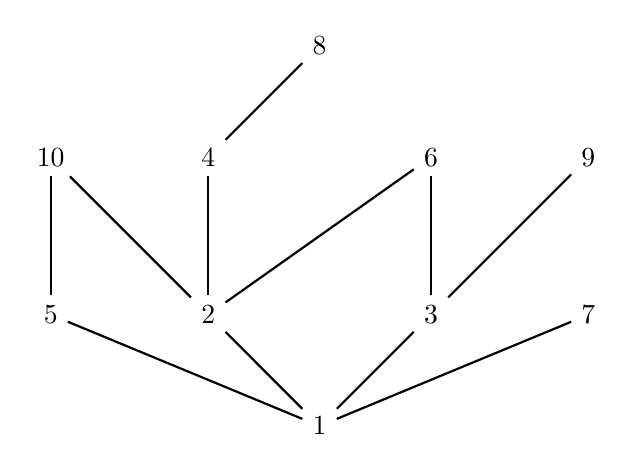
\begin{tikzpicture}[node distance={2cm}, thick]

\node (1) {$1$};
\node (2) [above left of=1] {$2$};
\node (5) [left of=2] {$5$};
\node (3) [above right of=1] {$3$};
\node (7) [right of=3] {$7$};
\node (4) [above of=2] {$4$};
\node (6) [above of=3] {$6$};
\node (9) [above of=7] {$9$};
\node (10) [above of=5] {$10$};
\node (8) [above right of=4] {$8$};

\draw (1) to (2);
\draw (1) to (3);
\draw (1) to (5);
\draw (1) to (7);
\draw (2) to (4);
\draw (2) to (6);
\draw (2) to (10);
\draw (3) to (6);
\draw (3) to (9);
\draw (5) to (10);
\draw (4) to (8);
\end{tikzpicture}
\caption{Relacija deljivosti za $\set{x\in\N\mid x\leq 10}$.}
\end{subfigure}
~
\begin{subfigure}[b]{0.48\textwidth}
\centering
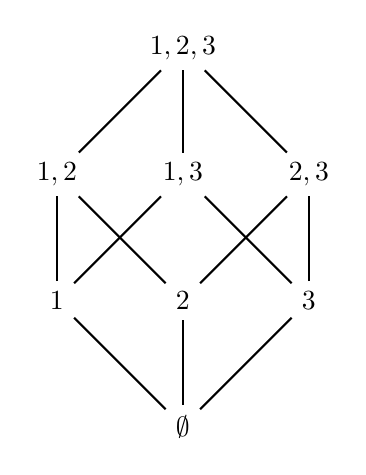
\begin{tikzpicture}[node distance={1.6cm}, thick]

\node (0) {$\emptyset$};
\node (1) [above of=0] {$\set{2}$};
\node (2) [left of=1] {$\set{1}$};
\node (3) [right of=1] {$\set{3}$};
\node (4) [above of=1] {$\set{1,3}$};
\node (5) [above of=2] {$\set{1,2}$};
\node (6) [above of=3] {$\set{2,3}$};
\node (7) [above of=4] {$\set{1,2,3}$};

\draw (0) to (1);
\draw (0) to (2);
\draw (0) to (3);
\draw (1) to (6);
\draw (1) to (5);
\draw (2) to (5);
\draw (2) to (4);
\draw (3) to (4);
\draw (3) to (6);
\draw (4) to (7);
\draw (5) to (7);
\draw (6) to (7);
\end{tikzpicture}
\caption{Relacija inkluzije za $\pot\set{1,2,3}$.}
\end{subfigure}

\caption{Hassejeva diagrama}
\end{figure}

\newpage

\subsection{Posebni elementi v delno urejenih množicah}

\begin{okvir}
\begin{definicija}
Naj $\leq$ delno ureja $A$ in naj bo $a\in A$.

\begin{enumerate}
\item $a$ je \emph{minimalen} v $A\iff\forall x\in A\colon(x\leq a\implies x=a)$
\item $a$ je \emph{maksimalen} v $A\iff\forall x\in A\colon(a\leq x\implies x=a)$
\item $a$ je \emph{prvi} ali \emph{najmanjši} element v $A\iff\forall x\in A\colon a\leq x$
\item $a$ je \emph{zadnji} ali \emph{največji} element v $A\iff\forall x\in A\colon x\leq a$
\end{enumerate}
\end{definicija}
\end{okvir}

\begin{trditev}
Naj bo $A$ delno urejena z $\leq$.

\begin{enumerate}
\item Vsak prvi element $A$ je minimalen.
\item Vsak zadnji element $A$ je maksimalen.
\item Če v $A$ obstaja prvi element, je enoličen.
\item Če v $A$ obstaja zadnji element, je enoličen.
\end{enumerate}
\end{trditev}

\obvs

\begin{trditev}
Naj bo $A$ linearno urejena z $\leq$. Potem je $a\in A$ prvi natanko tedaj, ko je minimalen in zadnji natanko tedaj, ko je maksimalen.
\end{trditev}

\obvs

\begin{opomba}
Naj $R$ delno ureja $A$ in naj bo $B\subseteq A$. Potem je $B$ delno urejena z \emph{zožitvijo} $R|_B=R\cap(B\times B)$ relacije $R$ na $B$.

\begin{enumerate}
\item Če ima $B\subseteq A$ prvi element, ga imenujemo tudi \emph{minimum}\index{Minimum in maksimum} množice $B$, ki ga označimo z $\min B$.
\item Če ima $B\subseteq A$ zadnji element, ga imenujemo tudi \emph{maksimum} množice $B$, ki ga označimo z $\max B$.
\end{enumerate}
\end{opomba}

\begin{definicija}
Naj bo $A$ delno urejena z $\leq$ in $B\subseteq A$.

\begin{enumerate}
\item $a\in A$ je \emph{zgornja meja}\index{Zgornja in spodnja meja} za $B$, če $\forall x\in B\colon x\leq a$
\item $a\in A$ je \emph{spodnja meja} za $B$, če $\forall x\in B\colon a\leq x$
\end{enumerate}
\end{definicija}

\begin{definicija}
Naj bo $A$ delno urejena z $\leq$.

\begin{enumerate}
\item Naj bo $M=\set{a\in A\mid\text{$a$ je zgornja meja za $B$}}$. Če ima $M$ prvi element, je to \emph{supremum}\index{Supremum in infimum} ali \emph{najmanjša (natančna) zgornja meja} za $B$ in ga označimo z $\sup B$.
\item Naj bo $M=\set{a\in A\mid\text{$a$ je spodnja meja za $B$}}$. Če ima $M$ zadnji element, je to \emph{infimum} ali \emph{največja (natančna) spodnja meja} za $B$ in ga označimo z $\inf B$.
\end{enumerate}
\end{definicija}

\begin{opomba}
Naj bo $B\subseteq A$ z delno urejenostjo.

\begin{enumerate}
\item Če ima $B$ zadnji element, je $\max B=\sup B$.
\item Če ima $B$ prvi element, je $\min B=\inf B$.
\end{enumerate}
\end{opomba}

\newpage

\subsection{Dobra urejenost}

\begin{okvir}
\begin{definicija}
Naj bo $R\subseteq A\times A$. Relacija $R$ \emph{dobro ureja}\index{Relacija!Dobra urejenost} množico $A$, če velja

\begin{enumerate}
\item $R$ delno ureja $A$
\item Vsaka neprazna podmnožica $B\subseteq A$ ima prvi element glede na $R_B$.
\end{enumerate}
\end{definicija}
\end{okvir}

\begin{trditev}
Vsaka dobra urejenost je linearna urejenost.
\end{trditev}

\begin{proof}
Ker ima $\set{a,b}$ prvi element za vse $a,b\in A$, je $R$ sovisna.
\end{proof}

\begin{opomba}
Vsaka končna linearno urejena množica je dobro urejena. Prav tako je $(\N,\leq)$ dobro urejena.
\end{opomba}

\begin{definicija}
Naj $R$ delno ureja $A$ in naj bo $V\subseteq A$. Če $R|_V$ linearno ureja $V$, je $V$ \emph{veriga}\index{Veriga} v $A$.
\end{definicija}

\begin{izrek}[O dobri urejenosti]\index{Izrek!O dobri urejenosti}
Za vsako množico $A$ obstaja relacija $R$, ki $A$ dobro ureja.
\end{izrek}

\begin{lema}[Zorn]\index{Lema!Zornova}
Naj relacija $R$ delno ureja $A$. Če ima vsaka veriga v $A$ zgornjo mejo, ima $A$ maksimalni element.
\end{lema}

\begin{opomba}
Aksiom izbire, izrek o dobri urejenosti in Zornova lema so v teoriji ZF med seboj ekvivalentni.
\end{opomba}

\newpage

\subsection{Mreža}

\begin{okvir}
\begin{definicija}
Delno urejena množica $A$ je \emph{mreža}\index{Mreža}, če
\[
\forall a,b\in A\colon (\exists\inf\set{a,b}\land\exists\sup\set{a,b}).
\]
\end{definicija}
\end{okvir}

\begin{posledica}
Vsaka linearno urejena množica je mreža.
\end{posledica}

\begin{proof}
Velja $\inf\set{a,b}=\min\set{a,b}$ in $\sup\set{a,b}=\max\set{a,b}$.
\end{proof}

\begin{opomba}
Dobra urejenost je poseben primer linearne urejenosti, ki je poseben primer mreže, ta pa je poseben primer delne urejenosti.
\end{opomba}

\newpage

\section{Moč množic}

\epigraph{">A lahko naredimo dokaz tega aksioma?"<}{---Jan Kamnikar}

\subsection{Množica naravnih števil}

\begin{okvir}
\textbf{Peanovi aksiomi:}\index{Aksiom!Peanovi}

\begin{enumerate}[label=P\arabic*.]
\item $0$ je naravno število.
\item Vsako naravno število $n$ ima točno določenega neposrednega naslednika $n'$.
\item Število $0$ ni naslednik nobenega števila.
\item Različni naravni števili imata različna neposredna naslednika.
\item Naj bo $L$ enomestni predikat. Če velja $L(0)$ in za vsako naravno število $n$ velja $L(n)\implies L(n')$, potem za vsako naravno število $n$ velja $L(n)$.
\end{enumerate}
\end{okvir}

V ZFC imamo naslednjo konstrukcijo:

\begin{definicija}
Za poljubno množico $A$ je $A'=A\cup\set{A}$ njen \emph{naslednik}\index{Naslednik}.
\end{definicija}

Za $0$ vzamemo kar $\emptyset$, kot naslednika števila pa vzamemo naslednika množice.

\begin{okvir}
\textbf{Aksiom regularnosti (AR):}\index{Aksiom!Regularnosti}
\[
\forall A\colon(A\ne\emptyset\implies\exists x\in A\colon x\cap A=\emptyset).
\]
Vsaka neprazna množica vsebuje element, s katerim ima prazen presek.
\end{okvir}

\begin{posledica}
Veljata naslednji trditvi:

\begin{enumerate}
\item $\forall a\colon a\not\in a$
\item $\forall a,b\colon\neg(a\in b\land b\in a)$
\end{enumerate}
\end{posledica}

\begin{proof}
Uporabimo aksiom regularnosti:

\begin{enumerate}
\item Naj bo $A=\set{a}$. Potem je $A\ne\emptyset$ in $a\cap A=\emptyset$. Če je $a\in a$, pa je $a\in a\cap A$, kar je protislovje.
\item Predpostavimo nasprotno. Po aksiomu o paru obstaja $A=\set{a,b}$. Tako je $a\in A\cap b$ in $b\in A\cap a$, kar je v protislovju z aksiomom regularnosti.\qedhere
\end{enumerate}
\end{proof}

\begin{definicija}
Množica $M$ je \emph{induktivna}\index{Množica!Induktivna}, če velja:

\begin{enumerate}
\item $\emptyset\in M$
\item $\forall x\in M\colon x'\in M$
\end{enumerate}
\end{definicija}

\begin{trditev}
Naj bo $A$ neprazna množica induktivnih množic. Potem je $\cap A$ induktivna množica.
\end{trditev}

\obvs

\begin{okvir}
\textbf{Aksiom neskončnosti (AN):}\index{Aksiom!Neskončnosti}

Obstaja induktivna množica.
\end{okvir}

\begin{izrek}
Obstaja natanko ena množica $\N$, da velja:

\begin{enumerate}
\item $\N$ je induktivna
\item $\forall A\colon(\text{$A$ induktivna}\implies \N\subseteq A)$
\end{enumerate}
\end{izrek}

\begin{proof}
Naj bo $M$ induktivna množica in $D=\set{A\subseteq M\mid\text{$A$ je induktivna}}$. Vzemimo $\N=\bigcap D$. Potem je $\N$ induktivna, za vsako induktivno množico $A$ pa je $A\cap M$ induktivna, zato je $\N\subseteq A\cap M$. Ni težko videti, da je to edina taka množica (v nasprotnem primeru je $\N_1\subseteq\N_2$ in $\N_2\subseteq\N_1$).
\end{proof}

\begin{izrek}[O indukciji]\index{Izrek!O indukciji}
Naj bo $L\subseteq\N$. Če velja

\begin{enumerate}
\item $0\in L$ in
\item $\forall n\in\N\colon (n\in L\implies n'\in L)$,
\end{enumerate}

je $L=\N$.
\end{izrek}

\begin{proof}
Vidimo, da je $L$ induktivna, zato je $\N\subseteq L$. Ker je $L\subseteq\N$, je $L=\N$.
\end{proof}

\newpage

\subsection{Relaciji $\sim$ in $\preccurlyeq$}

\begin{okvir}
\begin{definicija}
Množici $A$ in $B$ \emph{imata enako moč} ali sta \emph{ekvipolentni}\index{Ekvipolentnost}, če obstaja bijekcija $f\colon A\to B$. To zapišemo kot $A\sim B$.
\end{definicija}
\end{okvir}

\begin{trditev}
$\sim$ je ekvivalenčna relacija v razredu vseh množic $V$.
\end{trditev}

\obvs

\begin{okvir}
\begin{definicija}
$A$ ima \emph{manjšo ali enako moč} kot $B$, če obstaja injekcija $f\colon A\to B$. Pišemo $A\preccurlyeq B$.
\end{definicija}
\end{okvir}

\begin{trditev}
Za vse množice $A$, $B$ in $C$ velja

\begin{enumerate}
\item $A\subseteq B\implies A\preccurlyeq B$
\item $A\preccurlyeq B\implies \exists C\subseteq B\colon A\sim C$
\item $\preccurlyeq$ je refleksivna in tranzitivna 
\end{enumerate}
\end{trditev}

\obvs

\begin{izrek}[Schröder-Bernsteinov izrek]
Za poljubni množici $A$ in $B$ velja
\[
A\preccurlyeq B\land B\preccurlyeq A\implies A\sim B.
\]
\end{izrek}

\begin{izrek}
Če obstaja surjekcija $f\colon A\to B$, je $A\succcurlyeq B$.
\end{izrek}

\begin{proof}
Naj bo $f\colon A\to B$ surjekcija. Vsakemu elementu $y\in B$ lahko z aksiomom izbire priredimo en element praslike $\set{y}$. Dobimo funkcijo izbire
\[
g\colon B\to\bigcup_{y\in B}f^*(\set{y})=f^*\left(\bigcup_{y\in B}\set{y}\right)=f^*(B)=A,
\]
kjer je $g(y)\in f^*(\set{y})$ za vse $y\in B$. Ker je $f(g(y))\in\set{y}$, je $f\circ g$ injektivna, zato je $g$ injektivna.
\end{proof}

\begin{definicija}
$A$ ima \emph{strogo manjšo moč} kot $B$, če velja
\[
A\preccurlyeq B\land A\not\sim B.
\]
V tem primeru pišemo $A\prec B$.
\end{definicija}

\begin{izrek}[O trihotomiji]\index{Izrek!O trihotomiji}
Za vse $A,B$ velja natanko ena izmed naslednjih možnosti:

\begin{enumerate}
\item $A\prec B$
\item $A\sim B$
\item $A\succ B$
\end{enumerate}
\end{izrek}

\begin{posledica}
Za vse $A,B$ je $A\preccurlyeq B\lor B\preccurlyeq A$.
\end{posledica}

\newpage

\subsection{Končne in neskončne množice}

\begin{okvir}
\begin{definicija}[Dedekind]
Množica $A$ je \emph{neskončna}\index{Množica!Neskončna} natanko tedaj, ko
\[
\exists B\subset A\colon A\sim B.
\]
Sicer je $A$ \emph{končna}.	
\end{definicija}
\end{okvir}

\begin{izrek}
$A$ je neskončna natanko  tedaj, ko je $A\succcurlyeq\N$.
\end{izrek}

\begin{proof}
Če je $A$ neskončna, obstaja $B\subset A$, da je $A\sim B$. Naj bo $f\colon A\to B$ bijekcija. Naj bo $a\in A\setminus B$. Potem definiramo funkcijo $g\colon \N\to A$ na sledeč način:
\[
\forall n\colon g(n)=f^n(a).
\]
Ni težko videti, da je $g$ injektivna.

Če je $A\succcurlyeq\N$, obstaja injekcija $f\colon\N\to A$. Potem je
\[
\forall a\in A\colon g(a)=\begin{cases}
a, &a\not\in\mathcal{Z}_f
\\
f\left(f^{-1}(a)+1\right), &a\in\mathcal{Z}_f
\end{cases}
\]
injekcija iz $A$ v $A\setminus\set{f(0)}$.
\end{proof}

\begin{definicija}
Množica $A$ je \emph{števno neskončna}\index{Množica!Števna} natanko tedaj, ko je $A\sim \N$. $A$ je \emph{Števna}, če je končna ali števno neskončna. $A$ je \emph{neštevna} natanko tedaj, ko ni števna.
\end{definicija}

\begin{izrek}
Za vse $A$ velja:

\begin{enumerate}
\item $A$ je končna natanko tedaj, ko je $A\prec\N$
\item $A$ je števna natanko tedaj, ko je $A\preccurlyeq\N$
\item $A$ je števno neskončna natanko tedaj, ko je $A\sim\N$
\item $A$ je neskončna natanko tedaj, ko je $A\succcurlyeq\N$
\item $A$ je neštevna natanko tedaj, ko je $A\succ\N$
\end{enumerate}
\end{izrek}

\newpage

\subsection{Lastnosti števnih množic}

\begin{trditev}
Če obstaja surjekcija $g\colon\N\to A$, je $A$ števna.
\end{trditev}

\obvs

\begin{posledica}
Če lahko elemente $A$ razvrstimo v zaporedje tako, da vsak element $A$ v njem nastopi vsaj enkrat, je $A$ števna.
\end{posledica}

\begin{definicija}
Za družino $(A_\lambda)_{\lambda\in\mathcal{I}}$ pravimo, da je končna (neštevna, končna,
neskončna, števno neskončna), natanko tedaj, ko je takšna $\mathcal{I}$.
\end{definicija}

\begin{izrek}
Unija vsake števno neskončne družine števno neskončnih množic je števno neskončna.
\end{izrek}

\begin{proof}
Diagonalni argument.
\end{proof}

\begin{posledica}
Unija vsake števne družine števnih množic je števna.
\end{posledica}

\newpage

\subsection{Neštevne množice}

\begin{izrek}[Cantor]\index{Izrek!Cantorjev}
Za vsako množico $A$ je $\pot A\succ A$.
\end{izrek}

\begin{proof}
Ni težko najti injekcije $f\colon A\to\pot A$. Vzamemo lahko kar
\[
\forall x\in A\colon f(x)=\set{x}.
\]
Predpostavimo, da med $A$ in $\pot A$ obstaja bijekcija $g$. Zdaj vzamemo množico
\[
C=\set{x\mid x\not\in g(x)}.
\]
Ker je $C\subseteq A$, obstaja $x_0$, da je $C=g(x_0)$, kar je protislovje, saj velja
\[
x_0\in C\iff x_0\not\in g(x_0)\iff x_0\not\in C.\qedhere
\]
\end{proof}

\begin{posledica}
$\R\succ\N$, saj je $\R\sim\pot\N$.
\end{posledica}

\begin{posledica}
Obstaja neskončno zaporedje neskončnih množic različnih moči
\[
\N\prec\pot\N\prec\pot\pot\N\prec\dots
\]
Posebej označimo moč $\N$ z $\aleph_0$ in moč kontinuuma (moč $\R$) s $\mathfrak{c}=2^{\aleph_0}$.
\end{posledica}

\vspace{\fill}

\epigraph{">Auf Wiedersehen!"<}{---Jan Kamnikar}

\newpage
\printindex

\end{document}
